% --------------------------------------------------------------------------------------
% DOCUMENT METADATA - TO BE FILLED BY USER
% --------------------------------------------------------------------------------------
% --- Document Type ---
\newcommand{\DocumentType}{PRODUCT DESIGN DOCUMENT}    

% --- Project Identification ---
\newcommand{\ProjectRef}{25P01}                     
\newcommand{\ProjectTitle}{MORSE KEY}              

% --- Report Identification ---
\newcommand{\ReportRef}{R01}                           
\newcommand{\ReportTitle}{INITIAL DESIGN DOCUMENTATION} 
\newcommand{\DocVersion}{V01}                           

% --- Authoring and Assets ---
\newcommand{\AuthorName}{Nick McCleery}
\newcommand{\ReleaseDate}{\today}             
\newcommand{\LogoPath}{./assets/logo.pdf}     
\newcommand{\ReferenceFile}{25P01-R01V01-InitialDesignDocumentation.bib} 
% --------------------------------------------------------------------------------------
% END DOCUMENT METADATA
% --------------------------------------------------------------------------------------

% --------------------------------------------------------------------------------------
% DOCUMENT SETUP — GENERALLY TO BE LEFT UNCHANGED
% --------------------------------------------------------------------------------------
% Assemble shorthand
\newcommand{\ProjectFullRef}{\ProjectRef{} \ProjectTitle{}}
\newcommand{\ReportFullRef}{\ReportRef{}-\DocVersion{}}

% Fonts
\documentclass[10pt]{article}

\usepackage[utf8]{inputenc}
\usepackage[OT1]{fontenc}
\usepackage{ocr}

\usepackage{lmodern}
\renewcommand*\familydefault{\sfdefault}

% Set sections to use OCR-A1
\usepackage{sectsty}
\sectionfont{\ocrfamily\Large}
\subsectionfont{\ocrfamily\large}
\subsubsectionfont{\ocrfamily\normalsize}

% Core packages
\usepackage[english]{datetime2}
\usepackage{amsmath}
\usepackage{amssymb}
\usepackage{array}
\usepackage{booktabs}
\usepackage{enumitem}
\usepackage{fancyhdr}
\usepackage{float}
\usepackage{geometry}
\usepackage{graphicx}
\usepackage{longtable}
\usepackage{textcomp}
\usepackage{titlesec}
\usepackage{titling}
\usepackage{xcolor}

% Links
\usepackage[colorlinks=true,
            linkcolor=gray,
            citecolor=gray,
            urlcolor=gray
           ]{hyperref}

% Date
\DTMsetdatestyle{iso}

% Bibliography
\usepackage[backend=bibtex, style=ieee, citestyle=numeric-comp]{biblatex}
\addbibresource{\ReferenceFile}


% Set narrow page margins
\geometry{
  paper=a4paper,
  top=0.75in,
  bottom=0.75in,
  left=0.55in,
  right=0.55in,
  headsep=0.25in
}

% Remove paragraph indentation, add spacing between paragraphs
\usepackage{parskip}
\setlength{\parindent}{0pt}
\setlength{\parskip}{6pt}

% Header/Footer setup
\pagestyle{fancy}
\fancyhf{}
\renewcommand{\headrulewidth}{0.4pt}
\renewcommand{\footrulewidth}{0pt}
\fancyfoot[C]{\thepage}
\fancyhead[L]{\ocrfamily\small\ProjectFullRef}
\fancyhead[R]{\ocrfamily\small\ReportFullRef}
\setlength{\headheight}{20pt}

% Custom section style with horizontal lines
\titleformat{\section}
  {\ocrfamily\Large\bfseries}
  {\thesection}{1em}{}
  \titlespacing*{\section}
  {0pt}{1.5em}{1em}

\titleformat{\subsection}
  {\ocrfamily\large\bfseries}
  {\thesubsection}{1em}{}

\titleformat{\subsubsection}
  {\ocrfamily\normalsize\bfseries}
  {\thesubsubsection}{1em}{}

% Create a custom title command
\newcommand{\customtitle}{%
  \noindent
  \begin{minipage}[t]{0.65\textwidth}
    \vspace{-0.5cm}
    {\ocrfamily\Large\bfseries \DocumentType \par}
  \end{minipage}%
  \begin{minipage}[t]{0.35\textwidth}
    \flushright{}
    \includegraphics[width=0.5\textwidth]{\LogoPath}
  \end{minipage}

  \vspace{0.3cm}
  \hrule height 0.8pt
  \vspace{0.3cm}

  {\ocrfamily\bfseries\ProjectFullRef\par}
  {\ocrfamily\large\bfseries\ReportTitle\par}

  \vspace{0.5em}

  \begin{tabular}{@{}ll@{\hspace{2cm}}ll@{}}
    \ocrfamily\textbf{REPORT REF:} & \ocrfamily \ReportRef &
    \ocrfamily\textbf{AUTHOR:}     & \ocrfamily \AuthorName \\

    \ocrfamily\textbf{VERSION:}    & \ocrfamily \DocVersion &
    \ocrfamily\textbf{DATE:}       & \ocrfamily \ReleaseDate \\
  \end{tabular}

  \vspace{0.3cm}
  \hrule height 0.8pt
  \vspace{0.25cm}
}

% Create fullwidth table command
\newenvironment{fullwidthtable}
  {\begin{center}
   \begin{tabular*}{\textwidth}{@{\extracolsep{\fill}}ll@{}}}
  {\end{tabular*}
   \end{center}}


% Fold URLs
\usepackage{xurl}
\setlength{\emergencystretch}{1em}

\begin{document}
\vspace*{-1cm}
\thispagestyle{plain}
\customtitle{}


% --------------------------------------------------------------------------------------
% BEGIN REPORT CONTENT
% --------------------------------------------------------------------------------------
\section{Summary}

This document outlines the design process for a single part Morse key that employs a flexure hinge.
That process indicates that a pure-PLA, FDM-printed key should be suitable. The part should have an
upper arm section of 10mm x 3mm, with a cantilevered arm length of 80mm.

This design should provide for approximately 2mm of travel under 80gf actuation force, and offer a
Factor of Safety (FoS) of 16.

\section{Brief}
\subsection{Product Description}
A \texttt{single part} straight Morse key body that employs a flexure hinge. This product should be
considered a proof-of-concept intended for short duration demonstration purposes only.

\subsection{Initial Requirements}
The product must:
\begin{itemize}[leftmargin=*]
	\item When actuated, close an electrical circuit.
	\item When released, return to its open \texttt{home} position in a suitable timeframe.
	\item Require actuation force comparable to existing Morse keys or similar products.
	\item Provide sufficient mechanical durability for the intended product lifecycle.
	\item Include a stable base and/or appropriate mounting points to prevent unintended movement during
	      operation.
\end{itemize}

\subsection{Constraints}
The part must:
\begin{itemize}[leftmargin=*]
	\item Be manufacturable by FFF/FDM printing.
	\item Printed in PLA or PETG, or their CF-reinforced variants.
	\item Have total volume not exceeding 256x256x256mm.
	\item Have minimum wall thickness not less than 2mm.
	\item Have a maximum overhang angle of 45° without supports.
	\item Be manufacturable as a \texttt{single part} (as per product description). % Added from Markdown F6
\end{itemize}

\section{Research \& Requirements Development}
\subsection{Key Topics}
% This subsection was empty in the markdown.

\subsection{Actuation Force}

Reference information for morse key actuation force was found to be sparse. However, available
sources, \cite{ebay2025, eham2025}, list an adjustable morse key actuation range of 0--600gf, with
fixed actuation of $\approx$240gf. Based on intuitive assessment, this magnitude of actuation force
was felt to be greater than expected.

For comparison purposes, mechanical keyboard switches were investigated as alternative sources of
actuation force data. Both Keychron \cite{keychron2025} and Cherry MX \cite{cherry2025} publish
actuation force data for Cherry MX switch variants, and this data shows actuation forces ranging
from $\approx$45gf to $\approx$80gf.

\begin{figure}[H]
	\centering
	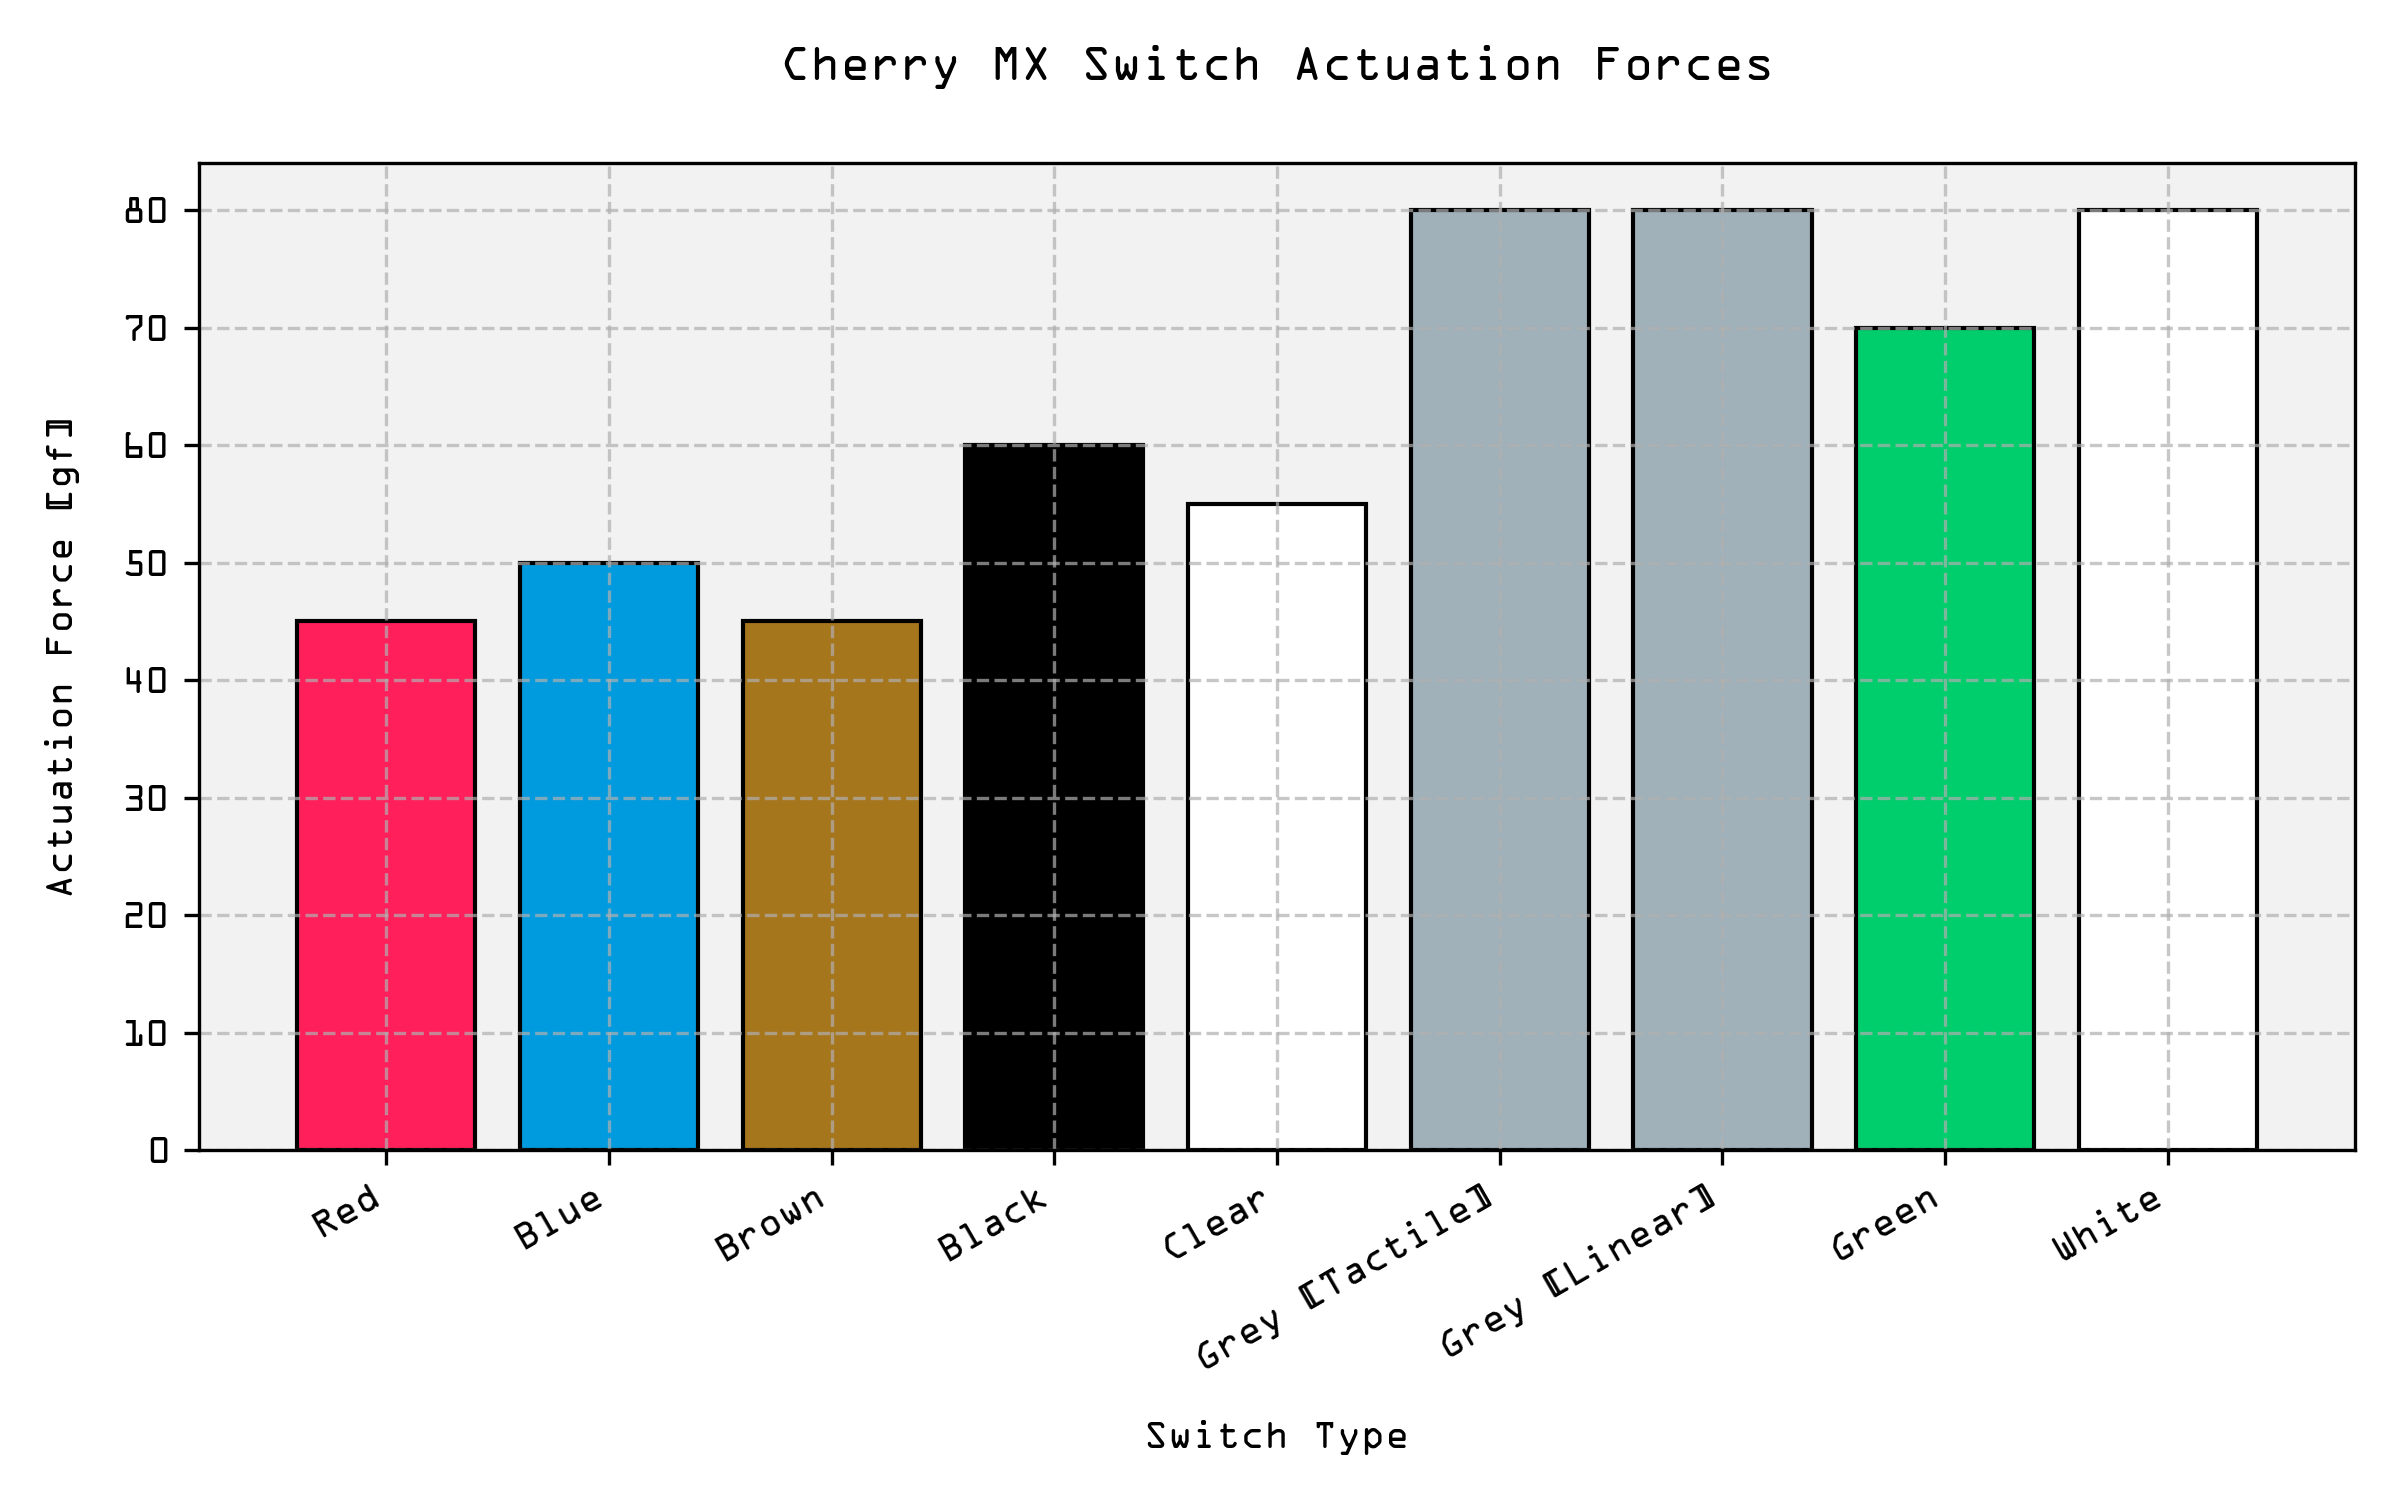
\includegraphics[width=0.75\textwidth]{./assets/01-cherry-mx-switches.png}
	\caption{Cherry MX Switch Actuation Force \cite{keychron2025, cherry2025}} % Added citations for context
	\label{fig:cherry-mx-switches}
\end{figure}

A hobbyist's blog post on the design of a manually milled morse key was also identified
\cite{giangrandi2025}. Though the post's author does not provide a target actuation force, they do
provide drawings and a nominal spring rate for the return spring employed in the design, from which
actuation forces can be calculated.

\autoref{fig:hobbyist-design} shows that the design is a second class lever, with the return
spring positioned between the pivot and the knob.

\begin{figure}[H]
	\centering
	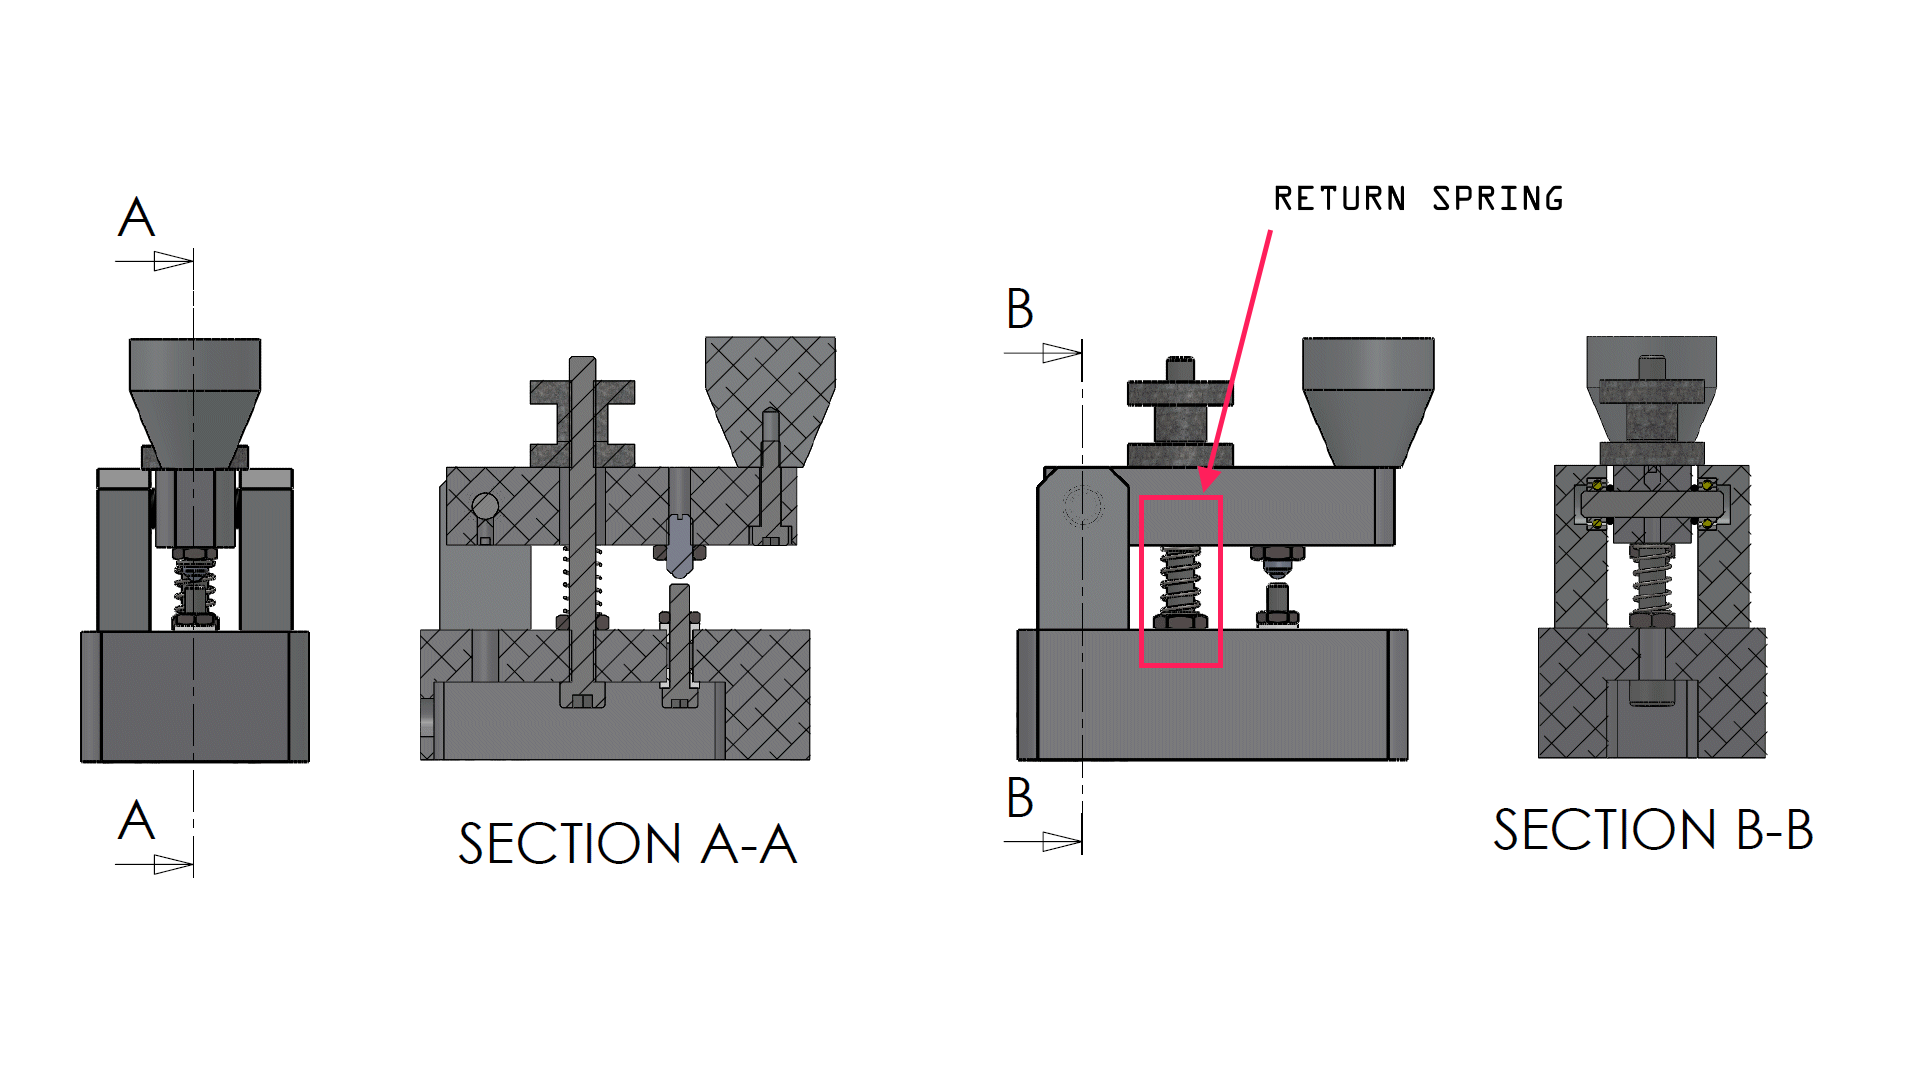
\includegraphics[width=\textwidth]{./assets/02-hobbyist-design.png}
	\caption{Hobbyist Morse Key Design \& Return Spring \cite{giangrandi2025}}
	\label{fig:hobbyist-design}
\end{figure}

Interrogation of the upper arm's drawing allows for relevant dimensions to be extracted and the
system analysed.

\begin{figure}[H]
	\centering
	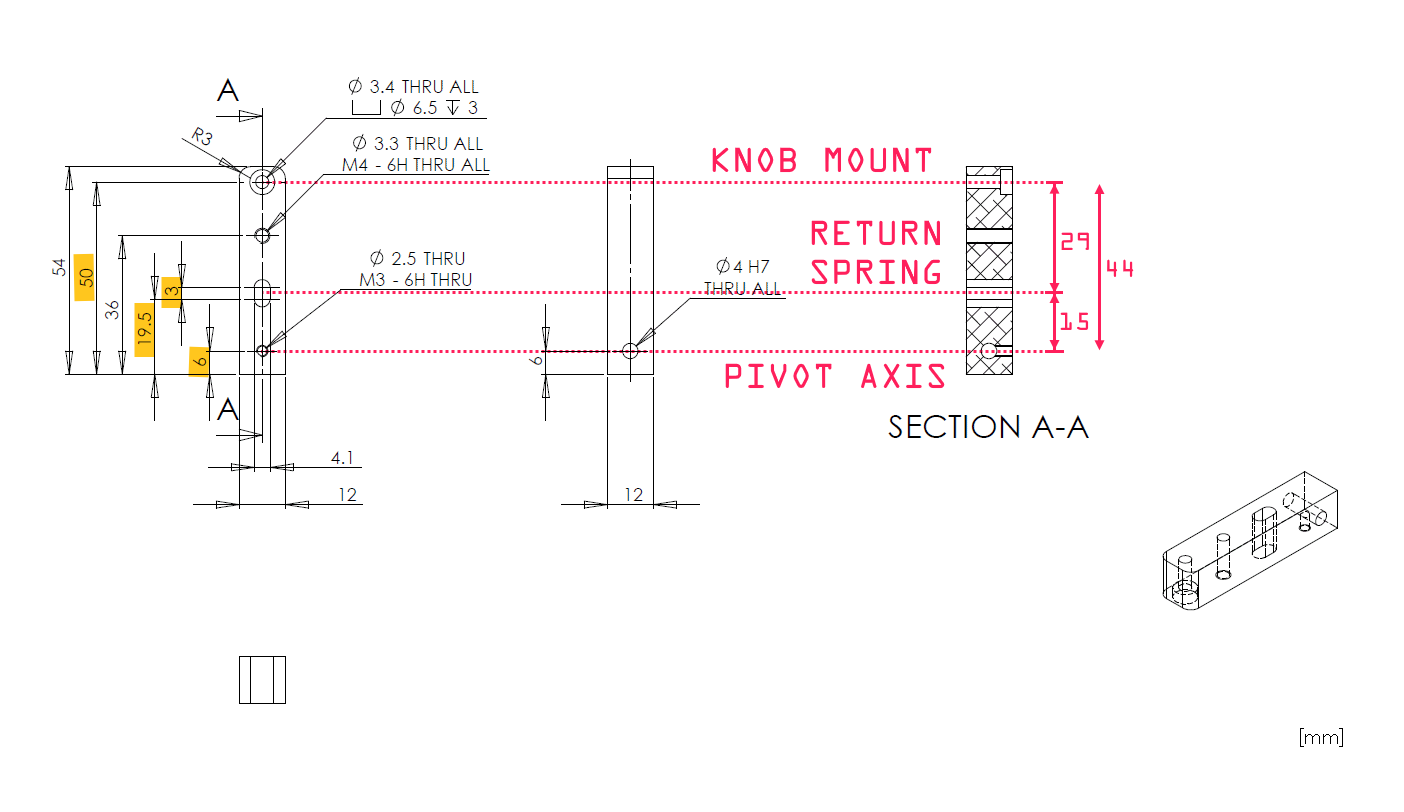
\includegraphics[width=\textwidth]{./assets/03-hobbyist-dims.png}
	\caption{Hobbyist Morse Key --- Critical Dimensions \cite{giangrandi2025}}
	\label{fig:hobbyist-dimensions}
\end{figure}

Simplifying, a free body diagram for the second class lever system is as given in
\autoref{fig:hobbyist-fbd}:

\begin{figure}[H]
	\centering
	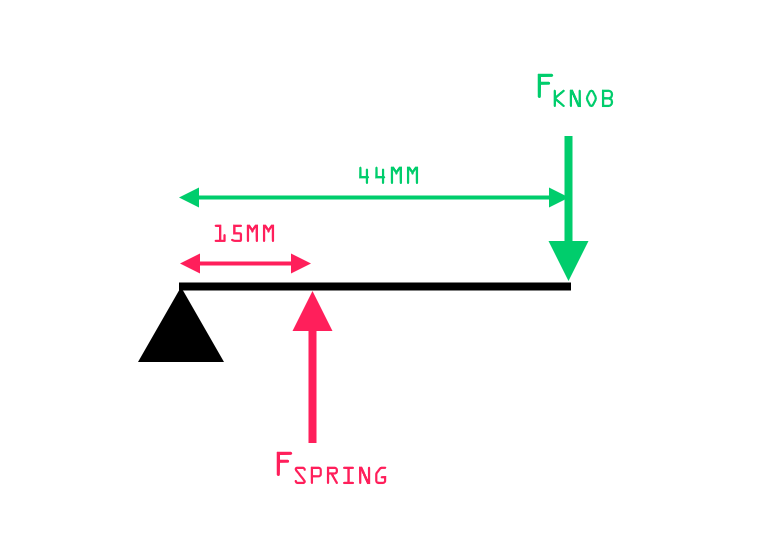
\includegraphics[width=0.5\textwidth]{./assets/04-fbd.png}
	\caption{Hobbyist Morse Key --- FBD}
	\label{fig:hobbyist-fbd}
\end{figure}

The key designer lists the spring's free length, $l_{\text{SpringFree}}$, as 14mm and its rate,
$k_{\text{Spring}}$, as 0.93N/mm \cite{giangrandi2025}. Further interrogation of the drawings also
shows that the spring will be subject to 1mm of preload compression when fitted. Combining these
values with the distances taken from the drawings, it becomes possible to compute the full set of
target values:

Constants:
\begin{align*}
	l_{Knob}          & = 44 \, \mathrm{mm}     \\
	l_{Spring}        & = 15 \, \mathrm{mm}     \\
	k_{Spring}        & = 0.93 \, \mathrm{N/mm} \\
	x_{SpringPreload} & = 1 \, \mathrm{mm}
\end{align*}

Apparent stiffness at knob:
\begin{align*}
	r_{MechanicalAdvantage} = \frac{l_{Knob}}{l_{Spring}} = \frac{44 \, \mathrm{mm}}{15 \, \mathrm{mm}}           & = 2.93                   \\
	k_{Installed}           = \frac{k_{Spring}}{r_{MechanicalAdvantage}^2} = \frac{0.93 \, \mathrm{N/mm}}{2.93^2} & = 0.108 \, \mathrm{N/mm}
\end{align*}

Force at knob to overcome spring preload:
\begin{align*}
	F_{Preload}       = k_{Spring} \cdot x_{SpringPreload} = 0.93 \, \mathrm{N/mm} \cdot 1 \, \mathrm{mm} & = 0.93 \, \mathrm{N}  \\
	F_{PreloadKnob}   = \frac{F_{Preload}}{r_{MechanicalAdvantage}} = \frac{0.93 \, \mathrm{N}}{2.93}     & = 0.317 \, \mathrm{N}
\end{align*}

As a confirmation step, mechanical advantage derived from lever arm length ratios can be compared
with `motion ratio' in terms of vertical displacement, $x$:

\begin{align*}
	\theta = 5^\circ = 0.0873 \, \mathrm{rad}                                                                                 \\
	x_{Knob} = l_{Knob} \cdot \sin(\theta) = 44 \, \mathrm{mm} \cdot \sin(0.0873 \, \mathrm{rad})     & = 3.83 \, \mathrm{mm} \\
	x_{Spring} = l_{Spring} \cdot \sin(\theta) = 15 \, \mathrm{mm} \cdot \sin(0.0873 \, \mathrm{rad}) & = 1.31 \, \mathrm{mm} \\
	r_{Motion} = \frac{x_{Knob}}{x_{Spring}} = \frac{3.83 \, \mathrm{mm}}{1.31 \, \mathrm{mm}}        & = 2.93                \\
	r_{Motion} \equiv{} r_{MechanicalAdvantage}                                                       & = 2.93
\end{align*}

Finally, converting to gram-force in the interest of comparability with values above, this would
equate to 32.3gf to overcome spring preload, with 11gf per mm of further travel---comparable in
magnitude with the Cherry MX keyboard switch actuation force.

\subsubsection{Recommendations}
While the actuation force derived from \cite{giangrandi2025} broadly aligns with the Cherry MX
switch data, commercially available morse keys are noted to have a stiffer operation. As a result,
it is recommended that target actuation force for the nominal travel distance be set at the highest
of the Cherry MX range: 80gf, or 0.78N.

\subsection{Travel Distance}
A preference for a gap of 0.2mm is noted in \cite{giangrandi2025}, but the design could accommodate
adjustment to a significantly larger value. \cite{electronicsnotes2025} recommends that novice
morse key users set a contact spacing of between 1.5mm and 2mm.

\subsubsection{Recommendations}
Given that novice users are advised to start with a contact spacing of $\approx$2mm, the finalised
design should provide adjustable spacing that accommodates travel distance in the range [0mm,
		2mm]---though larger gaps are acceptable.

\subsection{Contact Options}
Given the modest performance targets and initial requirements of the system, a simple steel
fastener should be adequate. \cite{giangrandi2025} uses a contact pair that is composed of a
conical point, stainless steel M4x10 and a socket head cap M3x16.

\subsubsection{Recommendations}
Stainless fastener contacts are assumed to be adequate for the system. Appropriate heat-set inserts
may be required, though given that there will be no service load on the fasteners, tapped holes in
the substrate may also be acceptable.

\subsection{Consolidated Requirements}
Based on both the initial brief requirements and the outcome of the background work detailed above,
categorised and consolidated product requirements are as follows:

\subsubsection{Performance Requirements}
\begin{itemize}[leftmargin=*]
	\item P1. Must provide actuation force of 80gf (0.78N) at the knob.
	\item P2. Must provide adjustable contact gap in range 0-2mm (larger gaps acceptable).
	\item P3. Must return to open position when released.
	\item P4. Return time should be suitable for Morse code operation.
	\item P5. Contact spacing should be adjustable with recommended initial setting of ~2mm.
\end{itemize}

\subsubsection{Electrical Requirements}
\begin{itemize}[leftmargin=*]
	\item E1. Must reliably close/open electrical circuit.
	\item E2. Contacts should be stainless steel fasteners (M4×10 conical point and M3×16 socket head cap
	      suggested).
	\item E3. May use heat-set inserts or tapped holes for contact mounting.
\end{itemize}

\subsubsection{Mechanical Requirements}
\begin{itemize}[leftmargin=*]
	\item M1. Must be stable during operation.
	\item M2. Must include appropriate mounting points.
	\item M3. Must provide sufficient mechanical durability for demonstration use.
	\item M4. Must employ a flexure hinge design (as per product description).
\end{itemize}

\subsubsection{Manufacturing Constraints}
\begin{itemize}[leftmargin=*]
	\item F1. Must be manufacturable by FFF/FDM printing.
	\item F2. Must be printed in PLA, PETG, or their CF-reinforced variants.
	\item F3. Maximum part volume: 256×256×256mm.
	\item F4. Minimum wall thickness: 2mm.
	\item F5. Maximum unsupported overhang angle: 45°.
	\item F6. Must be manufacturable as a \texttt{single part} (as per product description).
\end{itemize}

\subsubsection{Integration}
\begin{itemize}[leftmargin=*]
	\item I1. Should support incorporation of fastener-based contacts.
	\item I2. Should accommodate basic mounting/fastening requirements.
	\item I3. Should accommodate potential incorporation of heat-set inserts if needed.
\end{itemize}

\section{Concept Development} \label{sec:concept-development}
\subsection{Concept Exploration}
\subsubsection{Concept 1}
The first concept geometry employed a regular flexure (or living hinge design), using an arched and
notched geometry as described in \cite{sciendo2022}, which would have to be `folded' through
$\approx$180° to reach its service position.

\begin{figure}[H]
	\centering
	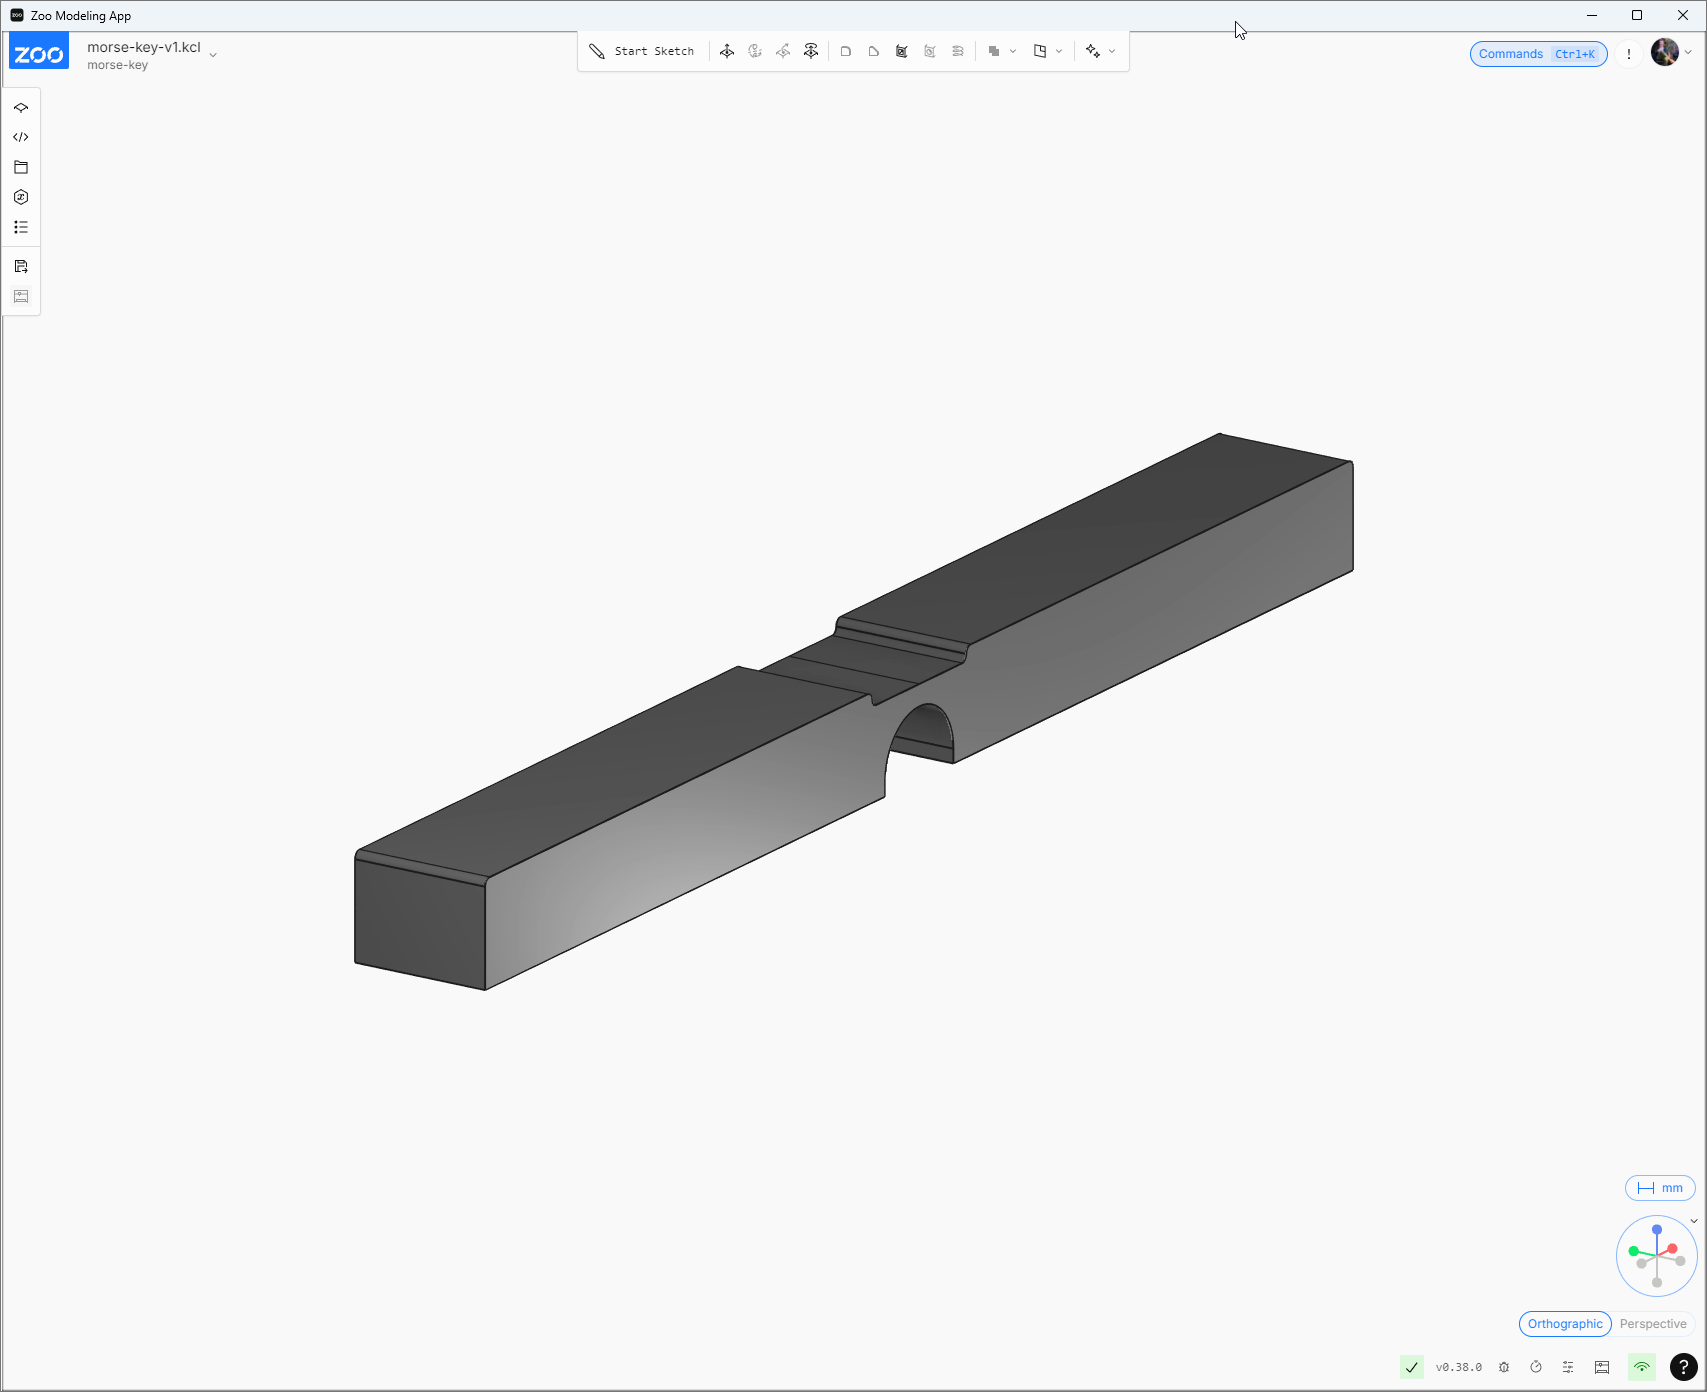
\includegraphics[width=\textwidth]{./assets/05-concept-01.png}
	\caption{Concept 1}
	\label{fig:concept-01}
\end{figure}

Though this concept is thought to be viable, the significant deformation between its
as-manufactured and in-service geometry was considered likely to make simulation and verification
of the design more challenging than necessary. It was also assumed that, though \cite{sciendo2022}
reports high fold cycle counts being achievable, that a design concept subject to less significant
deformation would likely be more robust.

\subsubsection{Concept 2}
A simpler concept was sought, ideally allowing for more straightforward analytical assessment of
stiffness, alongside more straightforward structural simulation. Accordingly, a simple C-shaped
profile was chosen.

\begin{figure}[H]
	\centering
	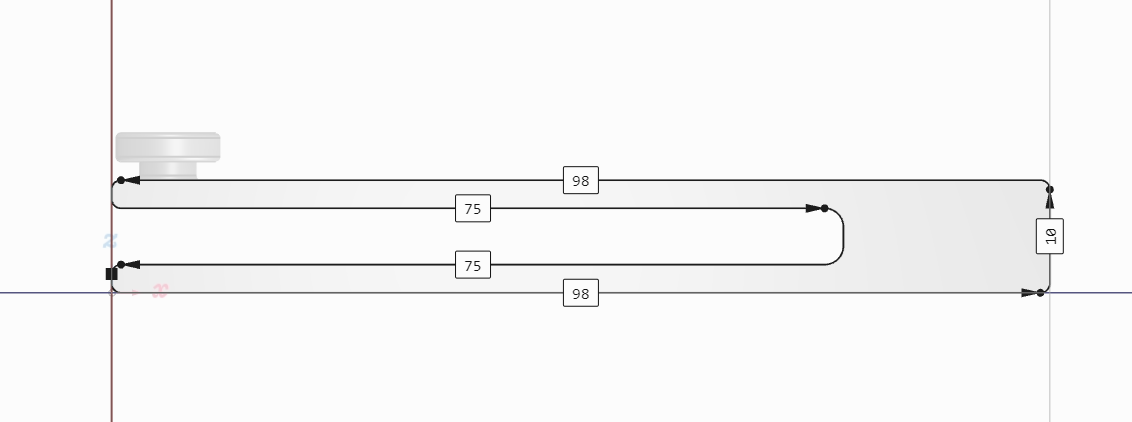
\includegraphics[width=0.75\textwidth]{./assets/06-concept-02.png}
	\caption{Basic Concept 2}
	\label{fig:concept-02}
\end{figure}

This profile should allow for application of cantilevered beam analogy to guide rough sizing. In
the event that the simple C-shaped profile cannot be rendered suitably compliant for the required
strength, this concept can also be adapted to use a `folded' approach, as demonstrated by
\cite{carson2024}. % Corrected citation key

\begin{figure}[H]
	\centering
	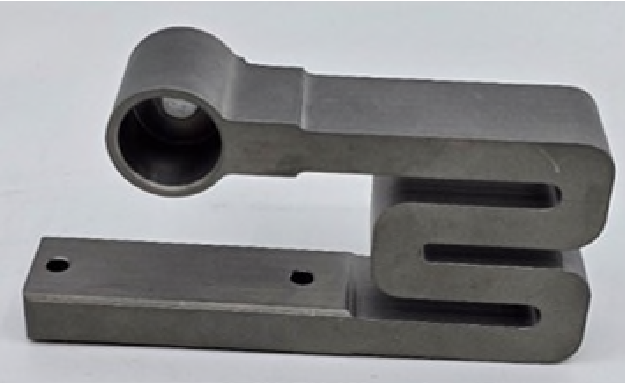
\includegraphics[width=0.5\textwidth]{./assets/07-folded.png}
	\caption{Folded Cantilevered Flexure \cite{carson2024}} % Corrected citation key
	\label{fig:folded-flexure}
\end{figure}

\subsection{Concept Selection} \label{sec:concept-selection}
The C-section concept was modelled analytically as a cantilevered beam with rectangular section,
point loaded at its extreme. Assuming a breadth of 10mm, peak deflection was computed for a range
of beam depths and cantilever lengths, and for two materials. In all cases, applied force was
assumed to be 0.78N.

The first material was Bambu Labs `basic' PLA filament \cite{bambulab_pla2025}. The second was the
carbon-fibre reinforced PLA variant \cite{bambulab_placf2025}. These offer properties as follows: % Corrected citation keys

\begin{table}[H]
	\centering
	\caption{Material Properties \cite{bambulab_pla2025, bambulab_placf2025}} % Added citations
	\label{tab:material-properties}
	\begin{tabular}{@{}lll@{}}
		\toprule
		\textbf{Property $\backslash$ Material} & \textbf{PLA}   & \textbf{PLA-CF} \\
		\midrule
		Bending Modulus                         & 2750 ± 160 MPa & 3950 ± 190 MPa  \\
		Bending Strength                        & 76 ± 5 MPa     & 89 ± 4 MPa      \\
		\bottomrule
	\end{tabular}
\end{table}

\begin{figure}[H]
	\centering
	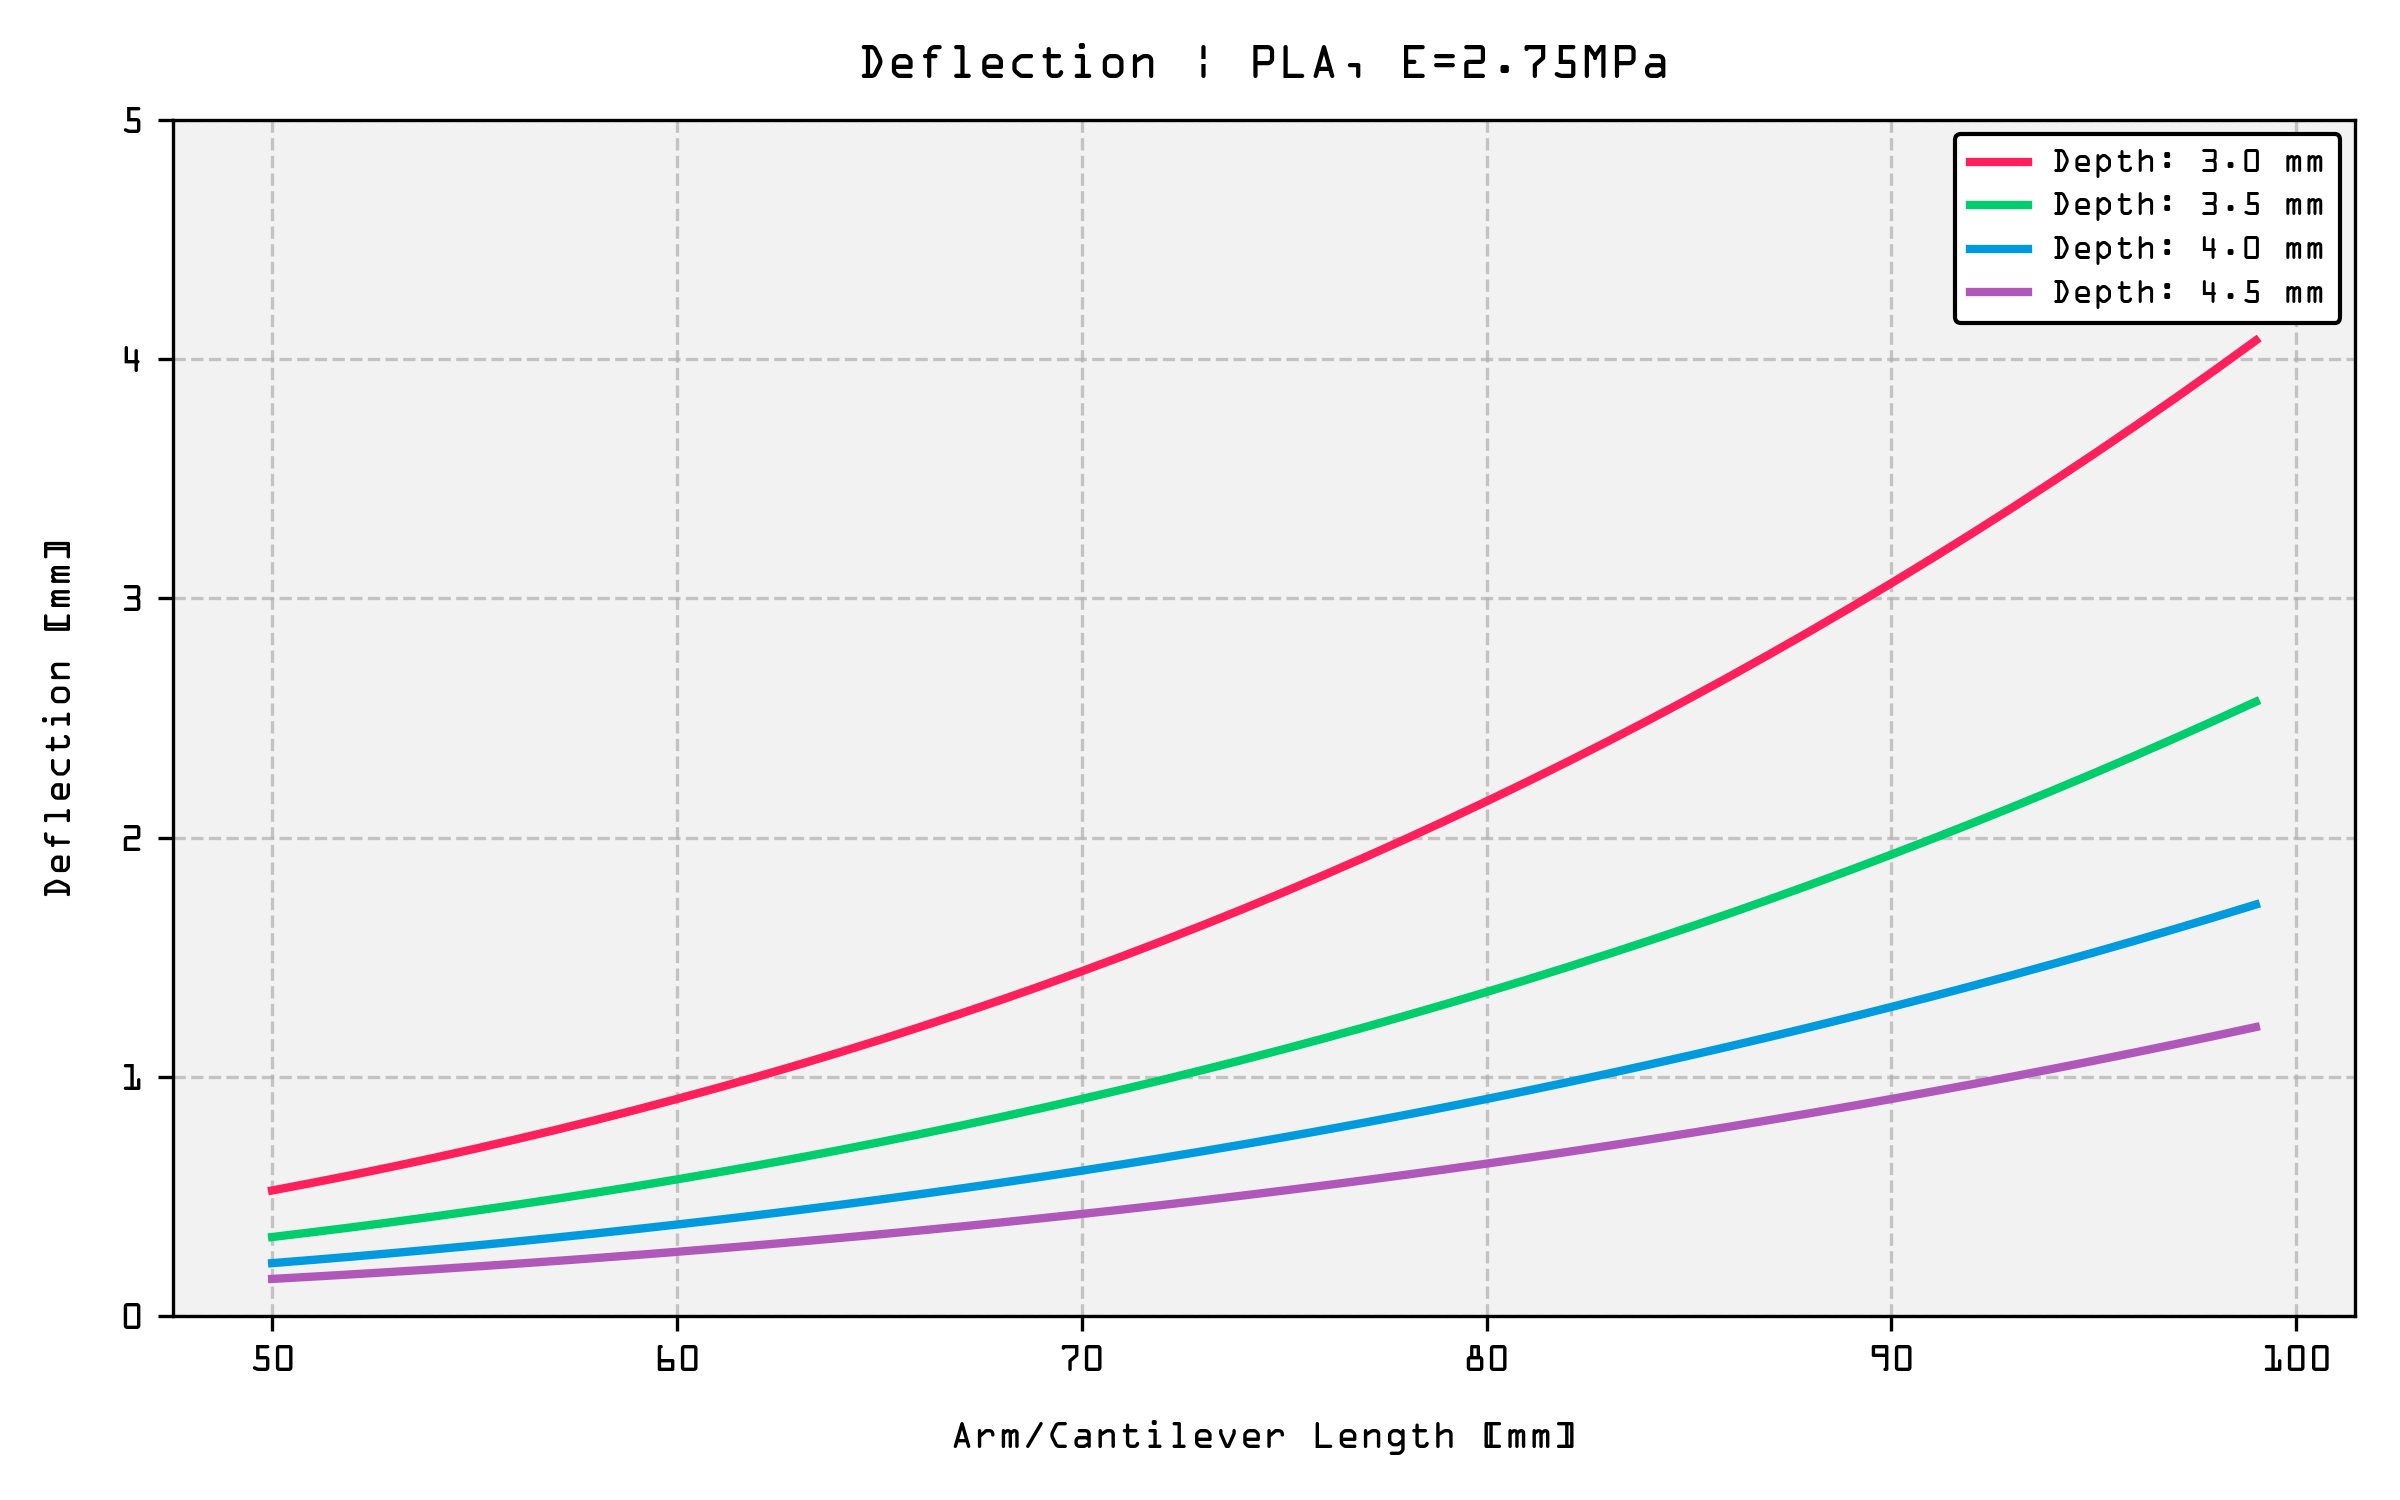
\includegraphics[width=\textwidth]{./assets/08-beam-deflection.png}
	\caption{PLA Cantilever Deflection}
	\label{fig:pla-deflection}
\end{figure}

\begin{figure}[H]
	\centering
	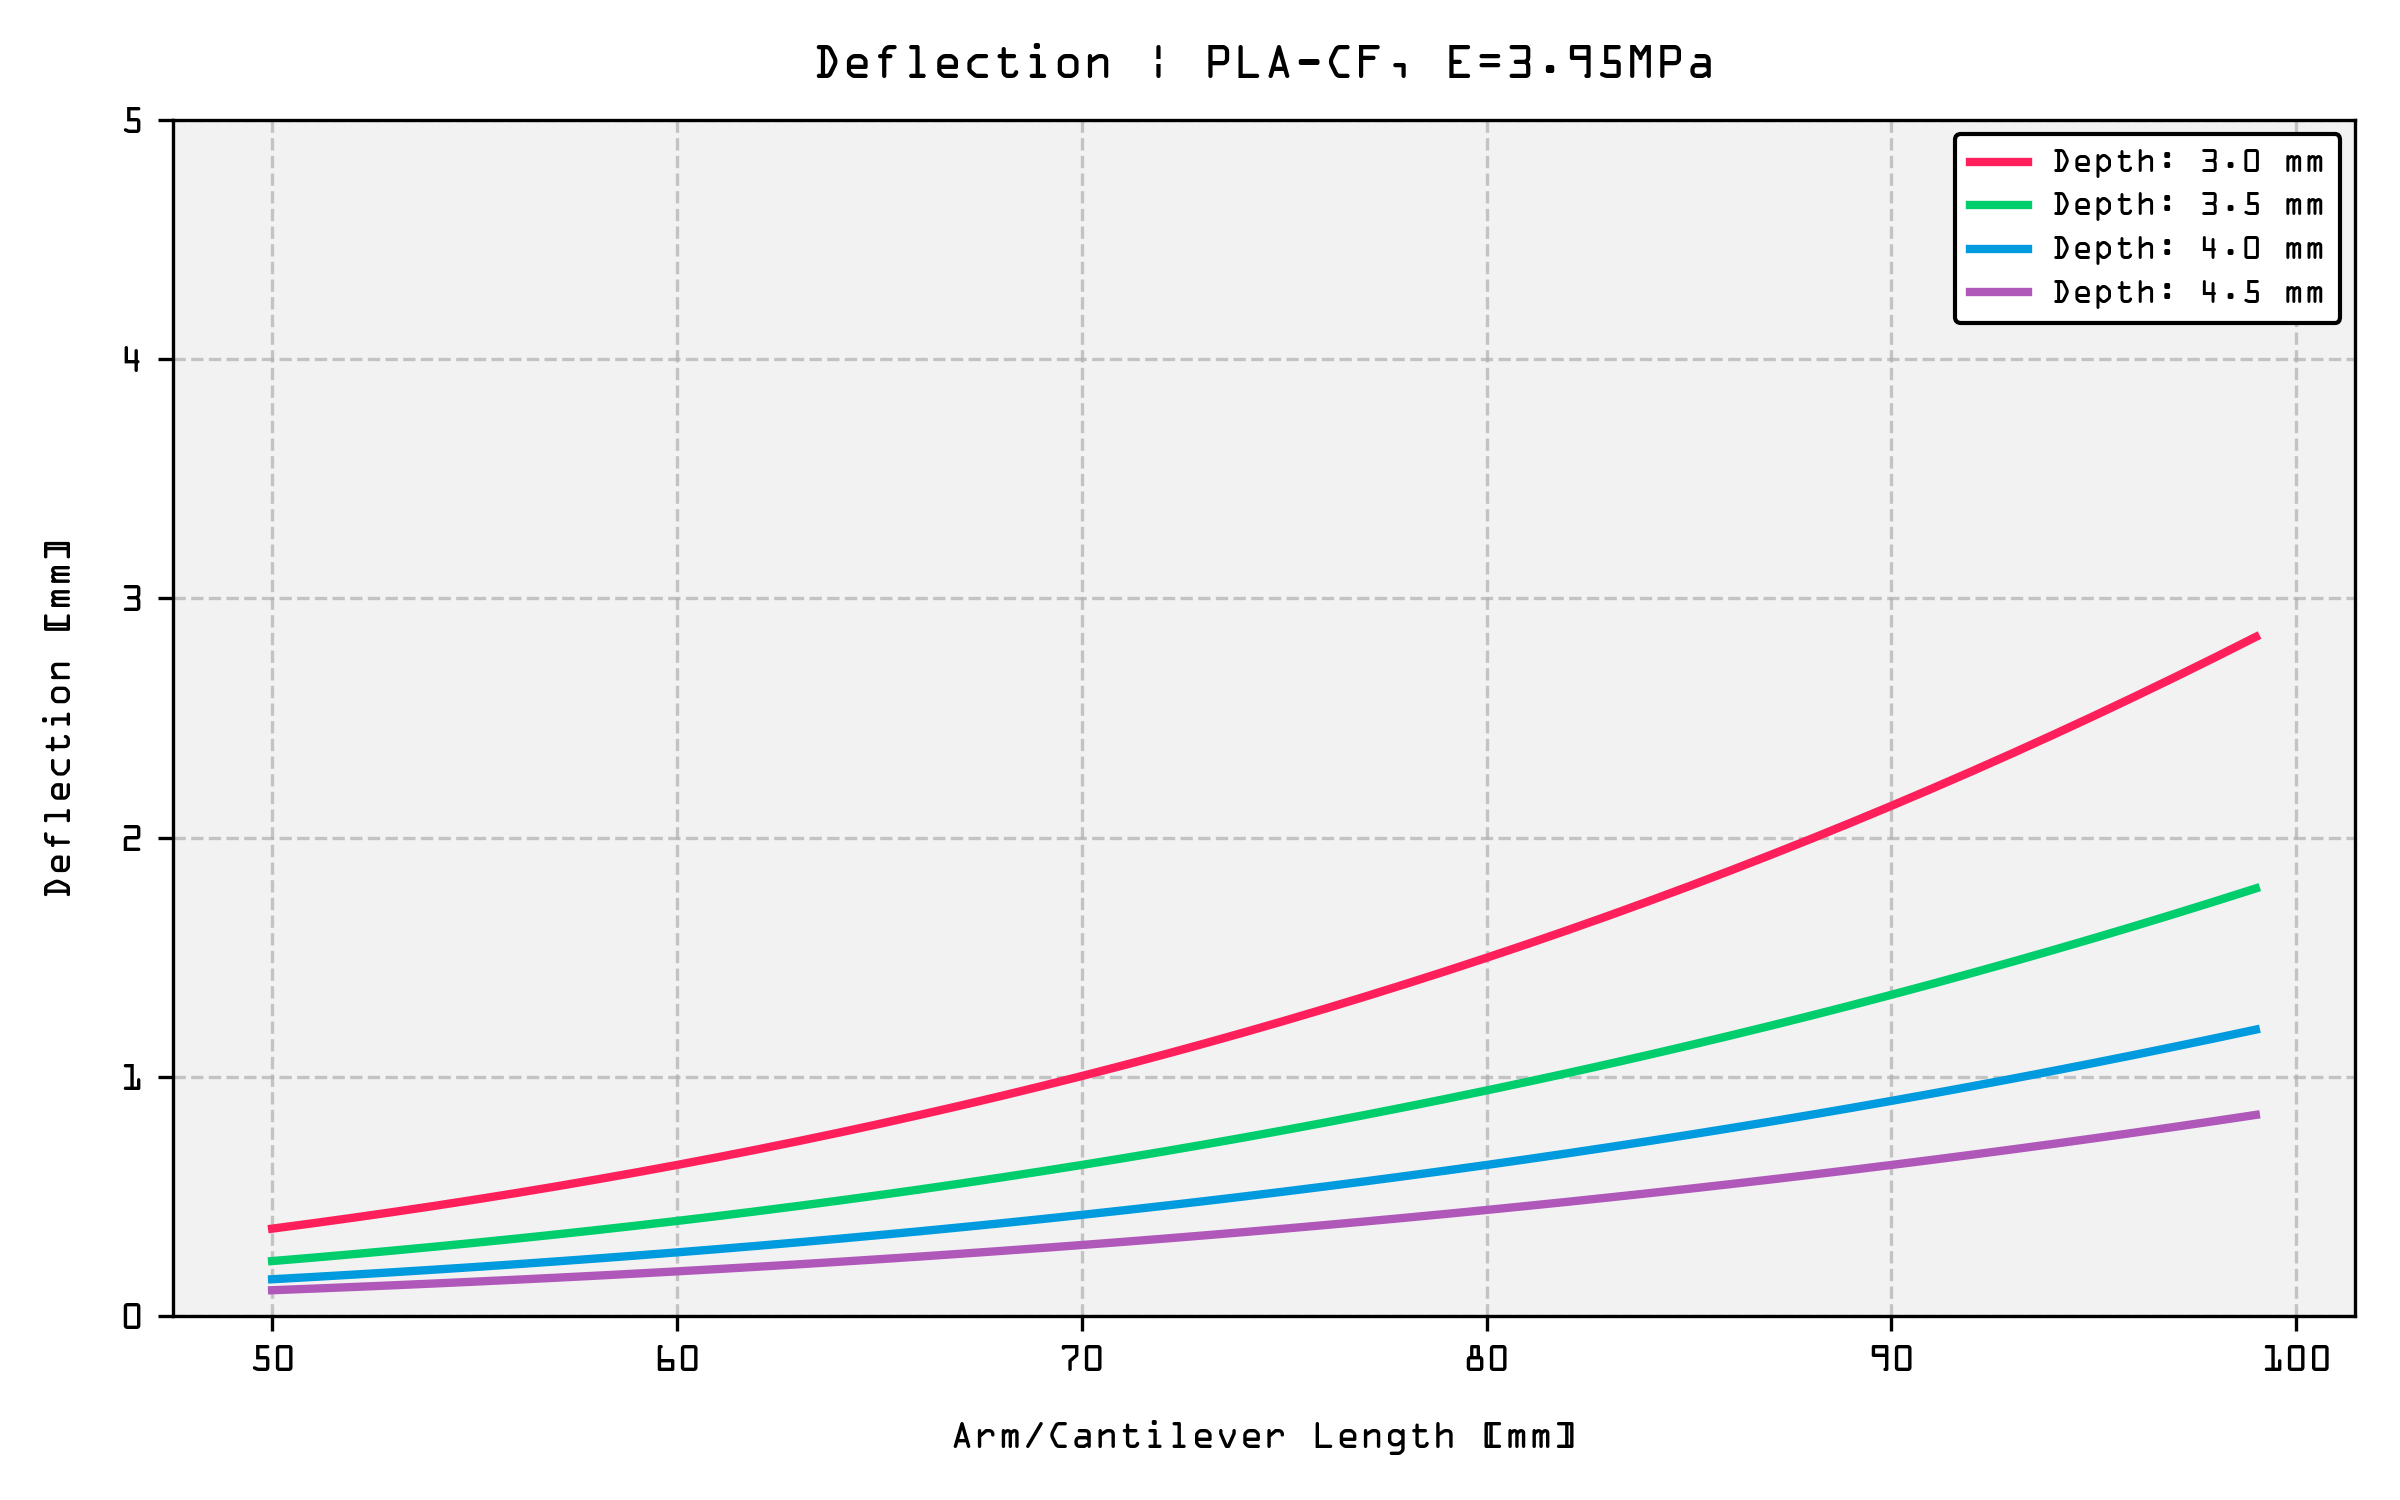
\includegraphics[width=\textwidth]{./assets/09-beam-deflection-cf.png}
	\caption{PLA-CF Cantilever Deflection}
	\label{fig:pla-cf-deflection}
\end{figure}

Based on these results, this concept is considered to be suitable when employing the basic PLA
filament. A rectangular beam depth of around 3mm should provide 2mm of displacement, and the
non-reinforced variant should be less likely to suffer a brittle failure mode.

\section{Design Development}
Based on the analytical work conducted during concept exploration
(\autoref{sec:concept-selection}), design work was begun assuming the upper arm would adopt:
\begin{itemize}[leftmargin=*]
	\item An 80mm cantilever.
	\item A 3x10mm rectangular section.
\end{itemize}

In pure PLA, making no consideration of print infill geometry or other print effects on structural
characteristics, this was predicted to offer $\approx$2mm of vertical displacement at the design
load of 0.78N.

\subsection{Key Design Features}
Beyond the cantilever dimension parameters, key features in the design were as follows:
\begin{enumerate}
	\item A large internal radius at the cantilever root.
	      \begin{itemize} \item Included in the interest of minimising stress in the region where the system will be subject to
		            bending. Though this feature was expected to reduce deformation at the upper arm's extremity under
		            load, no further adjustment to arm geometry was made. \end{itemize}
	\item Mounting lug pads.
	\item An integral knob for key operation.
\end{enumerate}

\begin{figure}[H]
	\centering
	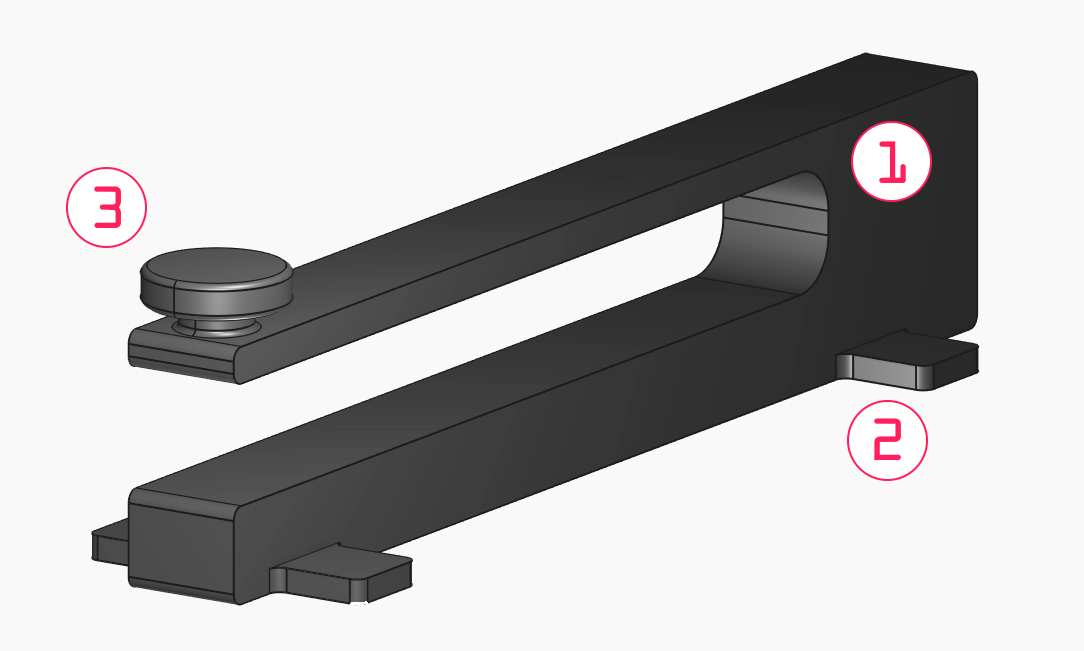
\includegraphics[width=0.75\textwidth]{./assets/10-key-design-features.png}
	\caption{Key Design Features}
	\label{fig:key-design-features}
\end{figure}

Note that some features were not included at this stage, e.g., mounting fastener holes, contact
arrangement holes, fillet radii at surface intersections etc.

\subsection{Material Selection}
PLA was deemed most suitable. Bambu Labs PLA filament offers adequate performance
\cite{bambulab_pla2025}. % Corrected citation key

\subsection{Manufacturing \& Assembly Considerations}
The part, as designed, is expected to require support structures during printing. Future
reconfiguration of knob and mounting lug arrangement may permit some reduction in support material
volume, but this is considered beyond the scope of this exercise.

Given that the part is intended to be subject to significant deformation in bending, print
direction must be considered. For maximum bending strength, the part should be printed such that
in-service bending load is applied perpendicular to print layers. For this part design, optimal
general print direction is assumed to be parallel to the lever arm central axis, depositing
filament in long horizontal passes \cite{protolabs2025}. This approach would also ensure that shear
loading does not induce delamination. % Corrected citation key

\subsection{Cost Considerations}
Not applicable; part to be printed in-house from commodity filament, mated with commodity
fasteners.

\section{Design Validation}
\subsection{Analytical Methods}
All analytical work conducted is described in \autoref{sec:concept-selection}; no further
analytical validation was undertaken.

\subsection{FEA/CFD}
PrePoMax~\cite{prepomax2025}, which uses CalculiX~\cite{calculix2025}, was used to validate the
deflection values presented in \autoref{fig:pla-deflection}.

\subsubsection{Methodology}
Relevant features (mounting and contact holes) were first finalised with FreeCAD, then a STEP file
was exported for use in PrePoMax. A simple model case was assembled as follows:
\begin{itemize}[leftmargin=*]
	\item Mesh: Second order tetrahedral throughout.
	\item Loads: A uniform pressure representing the design load (0.78N) applied to the top face of the knob.
	\item Boundary conditions: Fixed internal faces of mounting lug holes.
	\item Nonlinear geometric effects: Enabled.
	\item Material properties: As given in \autoref{sec:concept-selection}
	      (\autoref{tab:material-properties}), with Poisson's Ratio assumed to be 0.3.
\end{itemize}

Note that subdivision of the model to facilitate regional mesh type changes and/or boundary
condition refinement was not performed. In addition, the material was assumed to be solid and
isotropic (see: \autoref{sec:limitations}).

\begin{figure}[H]
	\centering
	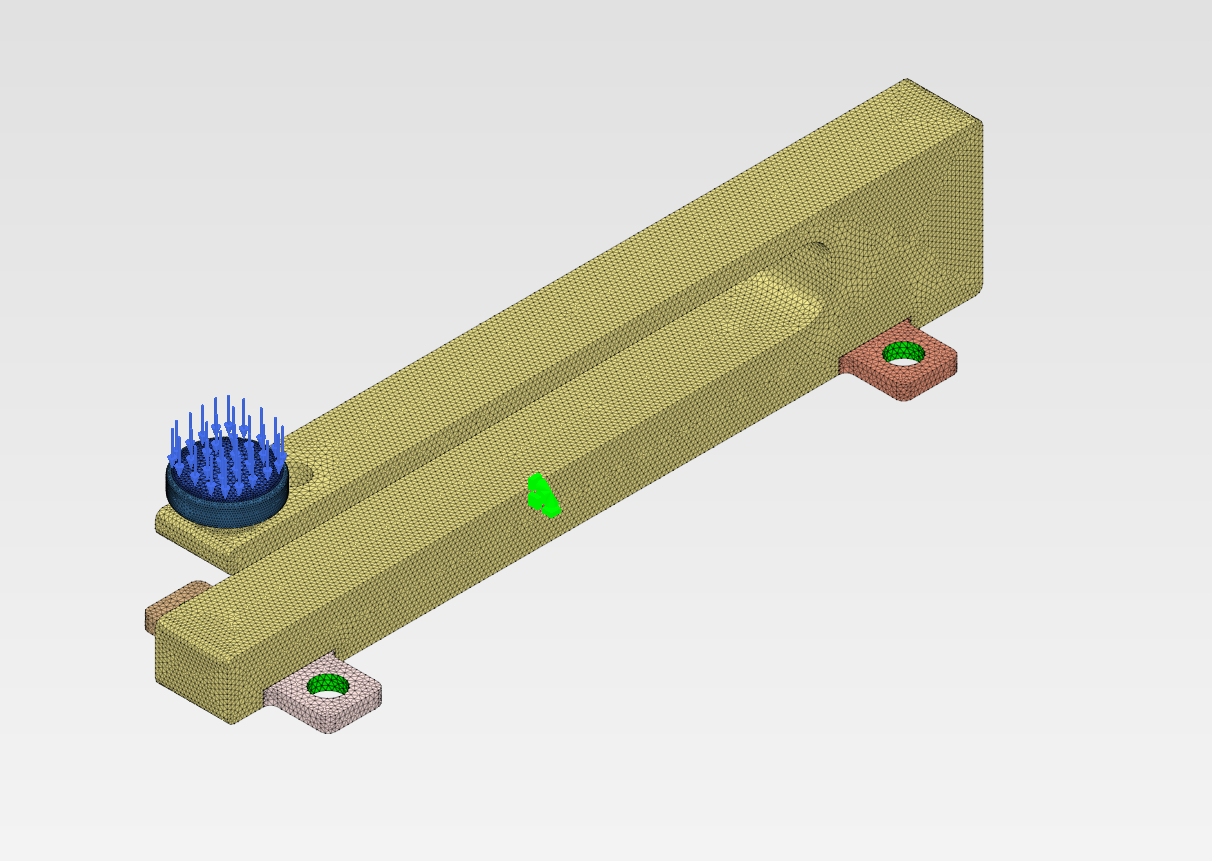
\includegraphics[width=\textwidth]{./assets/11-model-case.png}
	\caption{Model Case}
	\label{fig:model-case}
\end{figure}

\subsubsection{Mesh Convergence}
A simple mesh convergence exercise was completed:
\begin{itemize}[leftmargin=*]
	\item Iteration 1:
	      \begin{itemize}
		      \item Max element size: 5mm.
		      \item Min element size: 2mm.
	      \end{itemize}
	\item Iteration 2:
	      \begin{itemize}
		      \item Max element size: 2.5mm.
		      \item Min element size: 1mm.
	      \end{itemize}
	\item Iteration 3:
	      \begin{itemize}
		      \item Max element size: 1.25mm.
		      \item Min element size: 0.5mm.
	      \end{itemize}
	\item Iteration 4:
	      \begin{itemize}
		      \item Max element size: 0.625mm.
		      \item Min element size: 0.25mm.
	      \end{itemize}
\end{itemize}

Additionally, a model configured as in Iteration 3 had local mesh refinement applied, with element
size reduced to 0.25mm around key features.

Mesh convergence results are shown in \autoref{fig:mesh-convergence}, and local refinement is
illustrated in \autoref{fig:local-refinement}.

\begin{figure}[H]
	\centering
	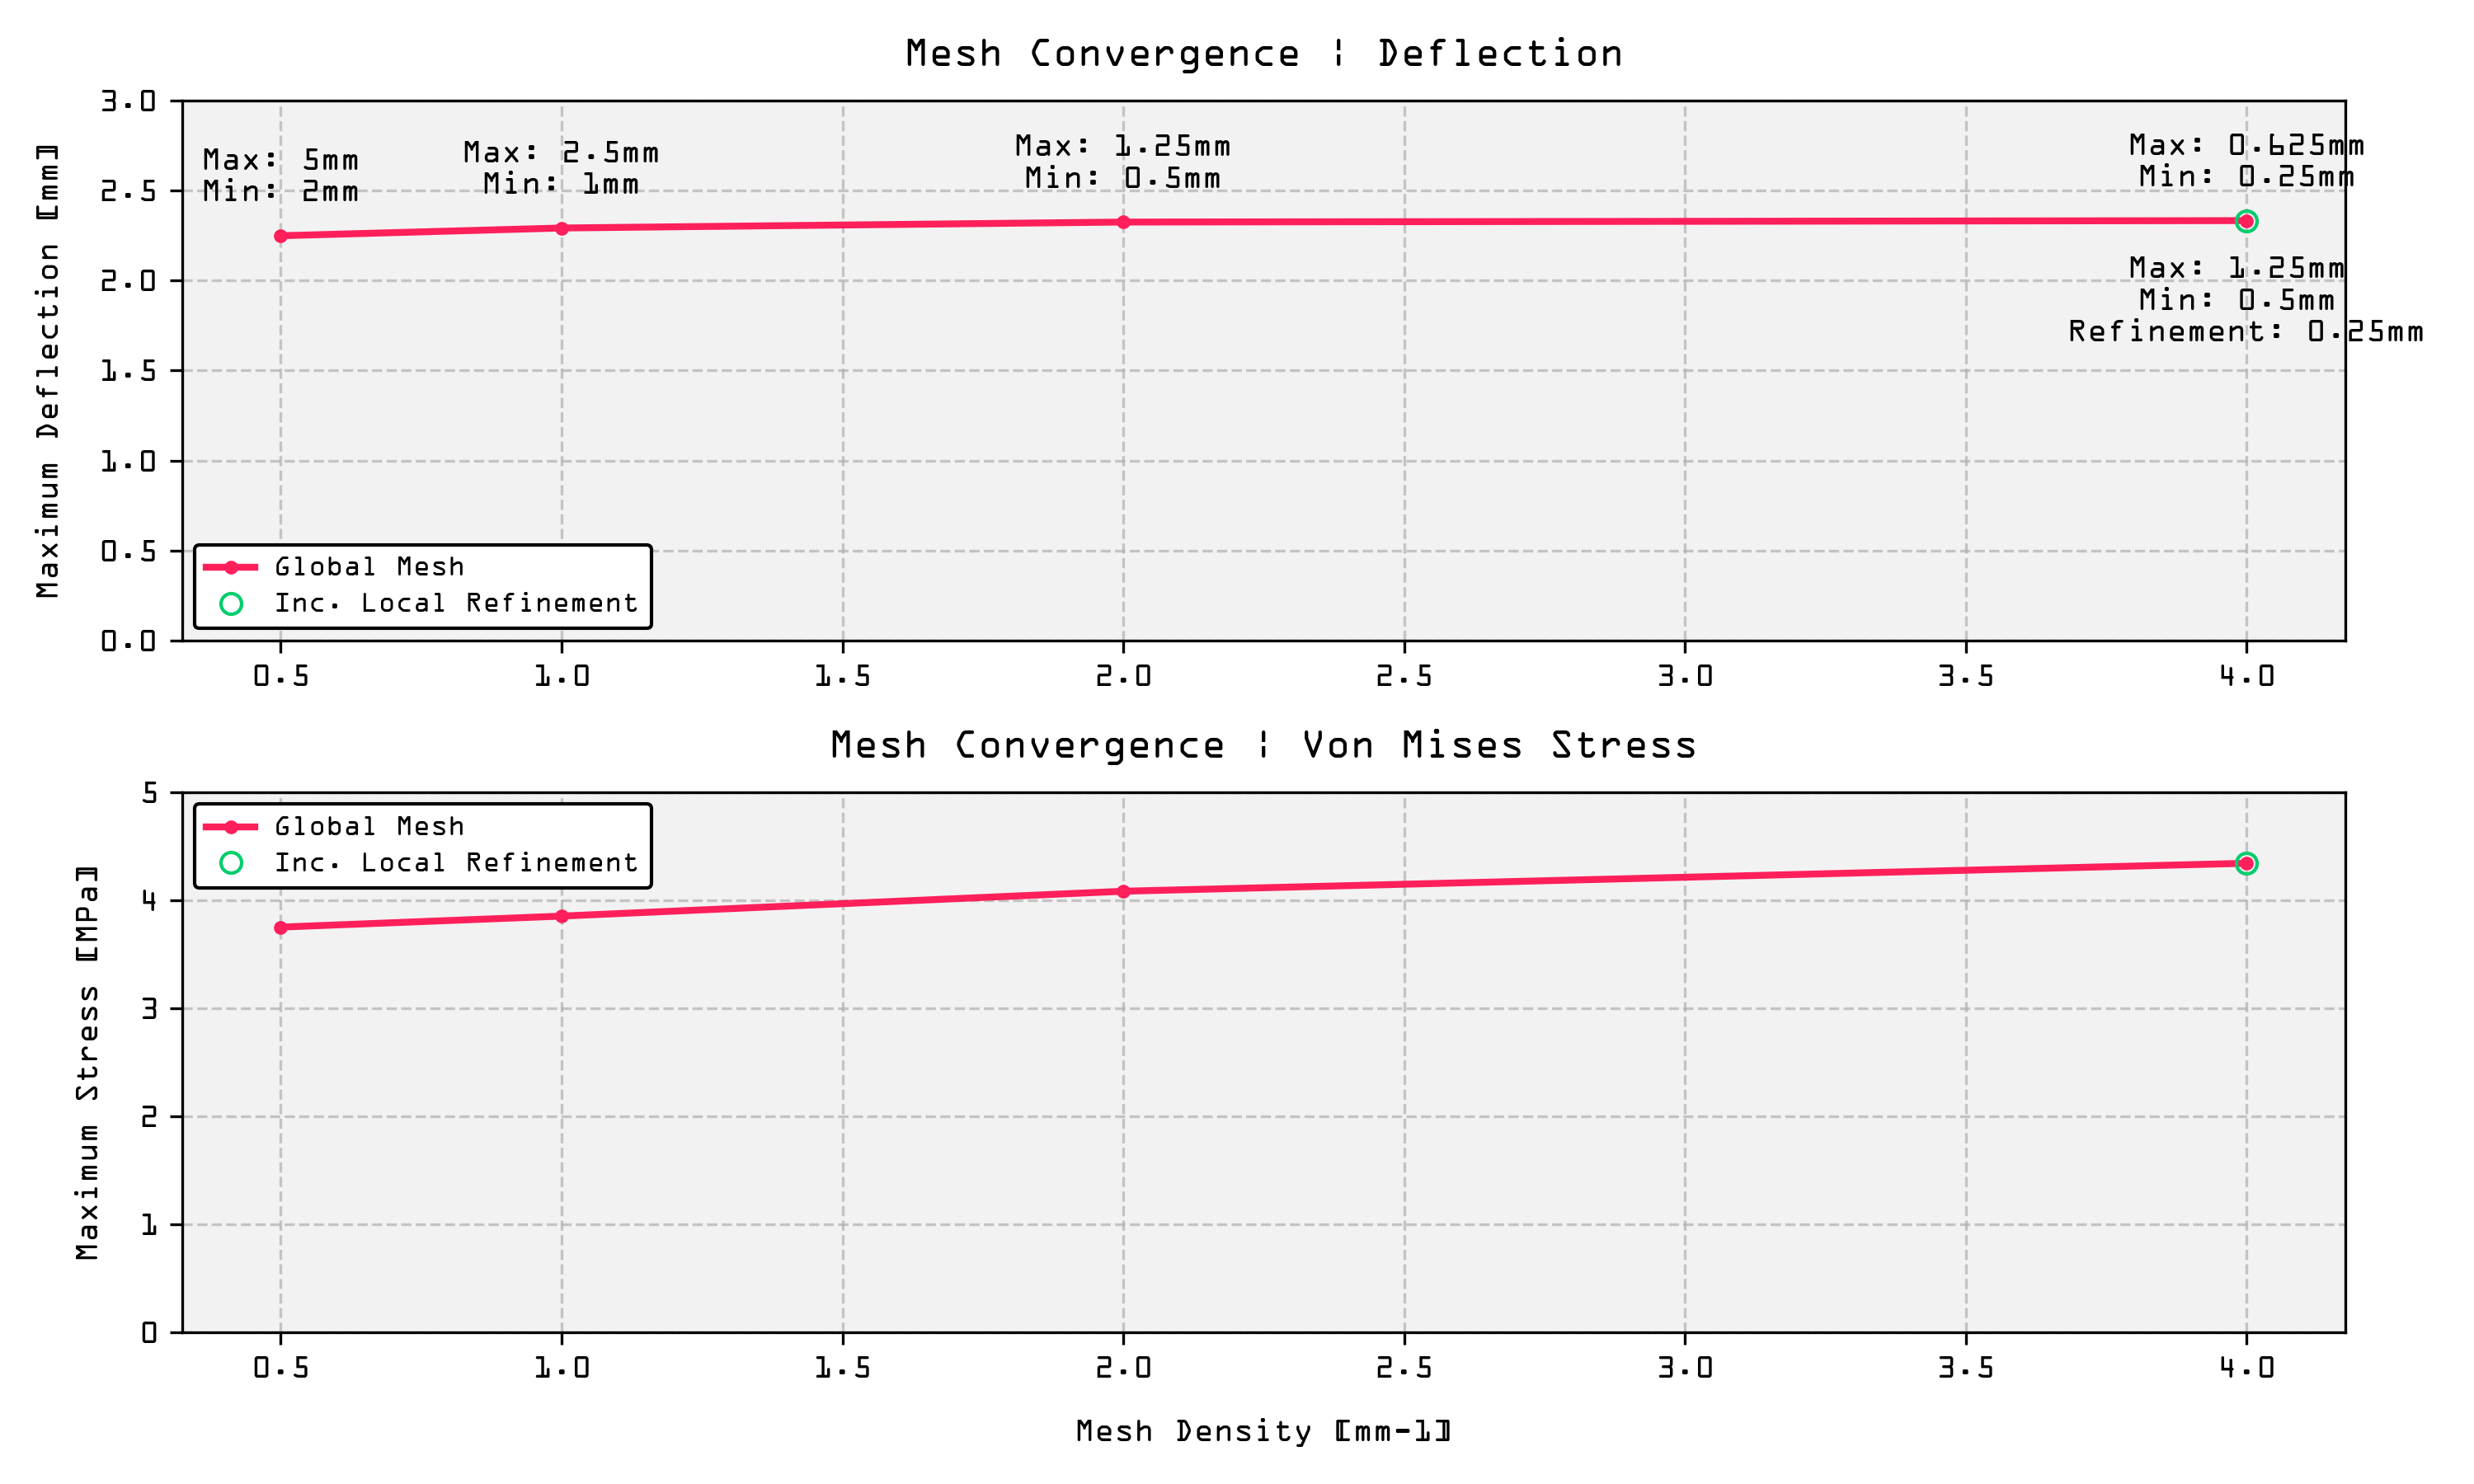
\includegraphics[width=\textwidth]{./assets/12-mesh-convergence.png}
	\caption{FEA Mesh Convergence}
	\label{fig:mesh-convergence}
\end{figure}

\begin{figure}[H]
	\centering
	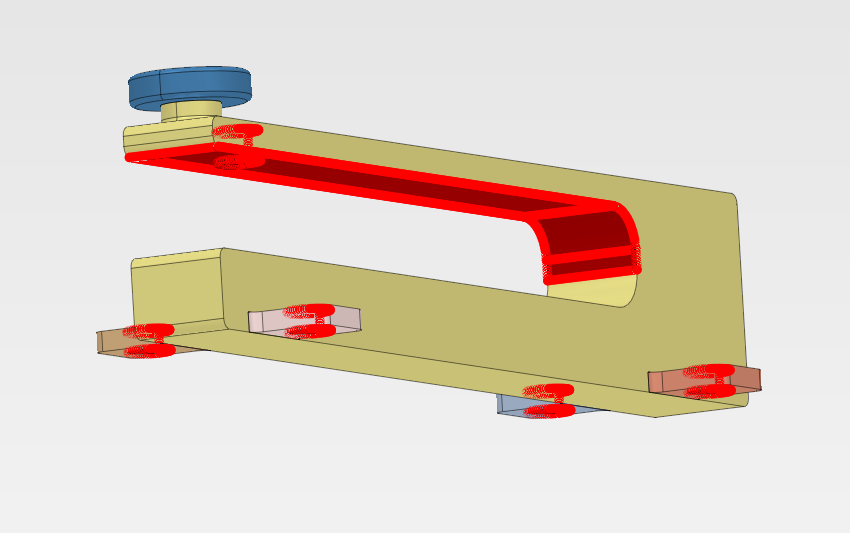
\includegraphics[width=\textwidth]{./assets/13-local-refinement.png}
	\caption{Local Mesh Refinement}
	\label{fig:local-refinement}
\end{figure}

\subsubsection{Results}
Iteration 4 and the locally refined Iteration 3 offer very close agreement in both peak deflection
and maximum Von Mises stress. In both cases, simulated maximum deflection was $\approx$2.33mm.
However, the node subject to maximum displacement relative to its starting point occurs at the knob
extremity most distant from the key's hinge.

Inspection of nodes in the vicinity of the knob centerline indicates simulated deflection of
$\approx$2.08mm, 96.7\% of the value predicted analytically. Given that the analytical approach
made no consideration of the radiused internal hinge, this result is considered to validate the
analytical method.

\begin{figure}[H]
	\centering
	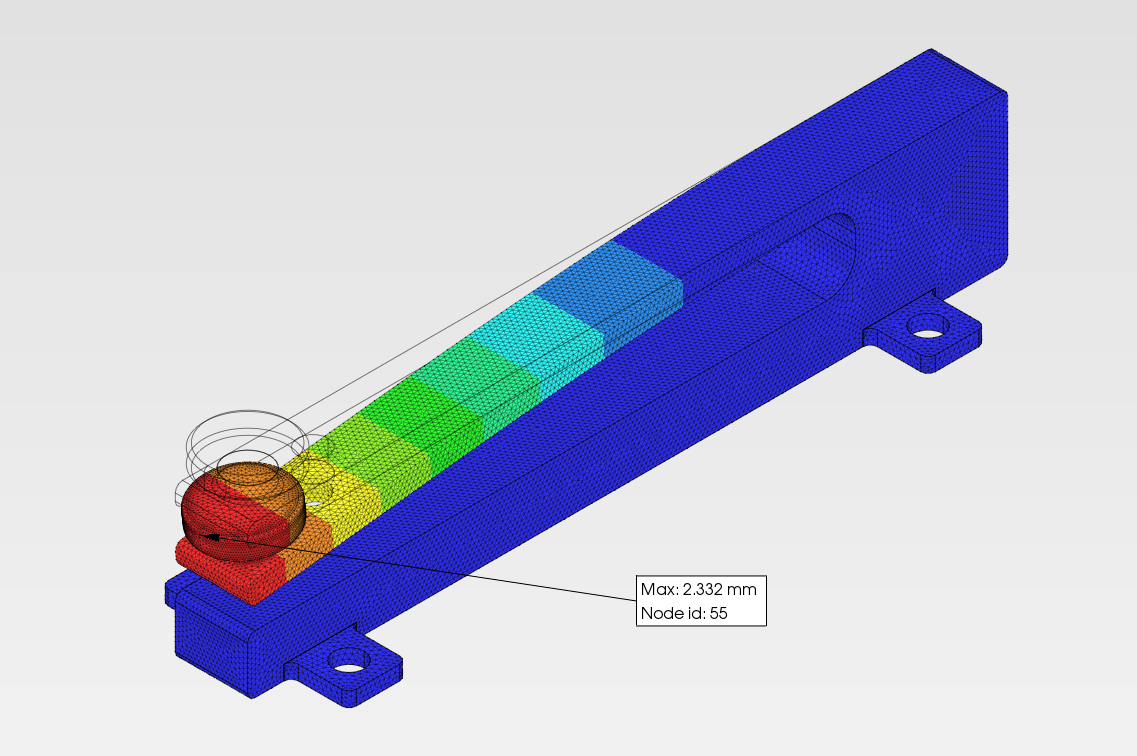
\includegraphics[width=\textwidth]{./assets/14-max-deflection.png}
	\caption{Iteration 4, Maximum Deflection}
	\label{fig:max-deflection}
\end{figure}

\begin{figure}[H]
	\centering
	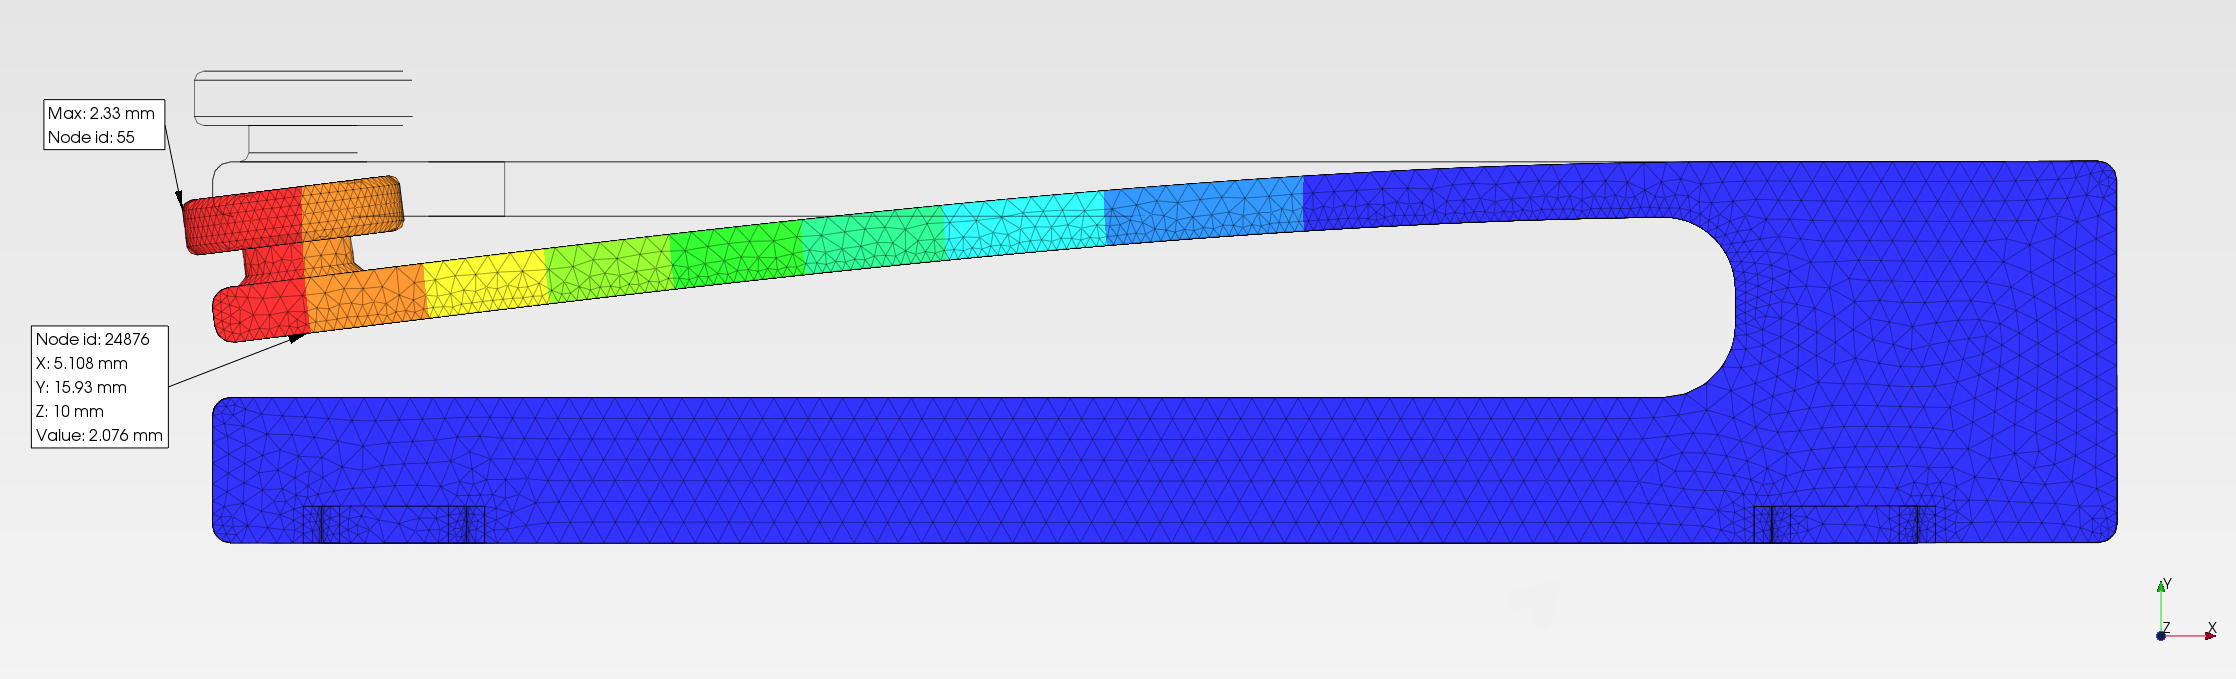
\includegraphics[width=\textwidth]{./assets/15-max-deflection-node.png}
	\caption{Iteration 3 Refined, Maximum Deflection at Key Node (Knob Centerline)}
	\label{fig:max-deflection-node}
\end{figure}

The values provided by \cite{bambulab_pla2025} indicate a bending strength of 76±5MPa for the basic
PLA filament. With respect to maximum bending stress, results indicate a peak Von Mises value of
4.346MPa---just 6\% of the lower bound of the material's bending strength. This gives a factor of
safety as follows: % Corrected citation key
\begin{align*}
	\text{Maximum bending strength}                        & = 76 \pm 5 \, \text{MPa} \\
	\text{Conservatively, } \sigma_{\text{Max}}            & =71 \, \text{MPa}        \\
	\\
	\text{Working Stress (FEA)}                            & = 4.346 \, \text{MPa}    \\
	\\
	\text{ FoS} = \frac{71\,\text{MPa}}{4.346\,\text{MPa}} & = 16.3
\end{align*}

Given the high FoS, the design is considered unlikely to fail in bending. For illustrative
purposes, simulated Von Mises stress is given in \autoref{fig:max-stress}.

\begin{figure}[H]
	\centering
	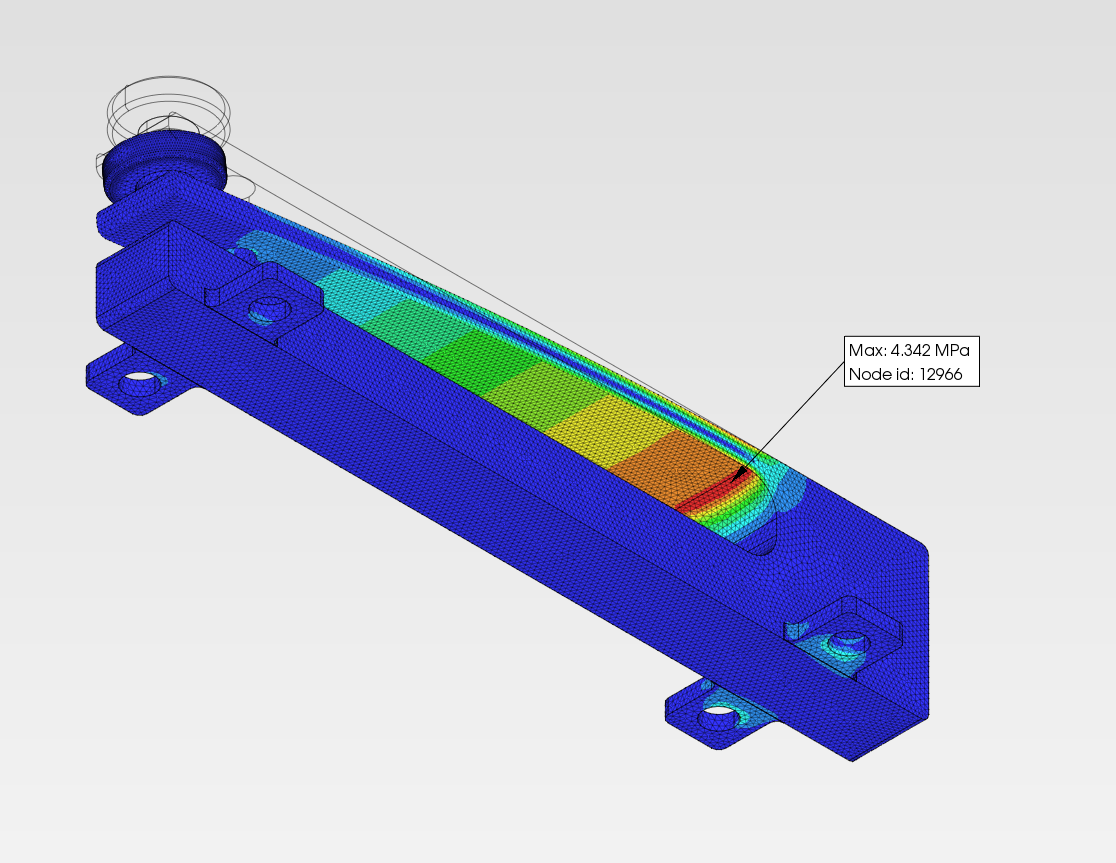
\includegraphics[width=\textwidth]{./assets/16-max-stress.png}
	\caption{Iteration 4, Maximum Von Mises Stress}
	\label{fig:max-stress}
\end{figure}

\section{Conclusion}
\subsection{Summary}
The documented design process suggests that a pure-PLA, FDM-printed key should be viable. Its upper
arm should be 10mm x 3mm, with a cantilevered arm length of 80mm.

This design should provide for approximately 2mm of travel under 80gf actuation force, and offer a
FoS of 16.

\subsection{Limitations} \label{sec:limitations}
\subsubsection{Contacts}
\begin{itemize}[leftmargin=*]
	\item Contact mechanics and wear were not considered.
\end{itemize}

\subsubsection{Material Behaviour}
\begin{itemize}[leftmargin=*]
	\item Materials assumed to be isotropic and ductile.
	\item Anisotropy arising from FDM print direction was not considered in analytical or finite element
	      methods.
	\item Raster orientation effects within layers (0°, 45°, 90° patterns) on mechanical response were
	      ignored.
	\item No work was undertaken to investigate any non-solid infill pattern.
	\item Void formation between extruded filaments was not modeled.
	\item Crystallinity variations due to cooling rates during printing were not considered.
	\item Residual stresses from thermal gradients during printing were not accounted for.
	\item Temperature effects were ignored.
	\item Hygroscopic effects (moisture absorption) on mechanical properties were not considered.
	\item Viscoelastic behavior (creep, stress relaxation) was not incorporated in the model.
	\item Strain-rate dependency of polymer response was not included.
\end{itemize}

\subsubsection{Analysis}
\begin{itemize}[leftmargin=*]
	\item Dynamic loading effects were ignored.
	\item Impact loading and sudden load application effects were not considered.
	\item Vibration effects and resonant frequencies were excluded from analysis.
	\item Cycle and fatigue behaviour were not considered.
	\item Mesh density sensitivity around critical features was not thoroughly investigated.
	\item Contact modeling between assembled parts was simplified.
\end{itemize}

\subsubsection{Manufacturing}
\begin{itemize}[leftmargin=*]
	\item FDM layer adhesion strength variation not considered.
	\item Extrusion parameters (temperature, multiplier, print speed) effects on mechanical properties were
	      not evaluated.
	\item Layer height influence on Z-direction strength was not investigated.
	\item Support structure impacts not considered.
	\item Environmental aging and UV degradation over time were not analyzed.
	\item Thin feature behavior relative to nozzle diameter was not specifically modeled.
	\item Sharp corner behavior and stress concentration effects specific to 3D printing were simplified.
	\item Shell-infill interface mechanics were not explicitly modeled.
\end{itemize}

\subsection{Further Work}
\subsubsection{Contacts}
\begin{itemize}[leftmargin=*]
	\item Analyse contact mechanics and optimise contact geometry.
	\item Model contact wear mechanisms.
	\item Evaluate alternative fastener materials and geometries.
\end{itemize}

\subsubsection{Material Analysis}
\begin{itemize}[leftmargin=*]
	\item Characterise printed PLA anisotropy through testing.
	\item Investigate optimal infill patterns and densities.
	\item Map operating temperature effects.
\end{itemize}

\subsubsection{FEA Refinement}
\begin{itemize}[leftmargin=*]
	\item Implement hexahedral/transfinite mesh.
	\item Apply contact boundary conditions at mounting points.
	\item Incorporate anisotropic material properties.
	\item Model dynamic loading effects.
\end{itemize}

\subsubsection{Manufacturing Development}
\begin{itemize}[leftmargin=*]
	\item Optimise print orientation for layer adhesion.
	\item Develop support structure strategy.
	\item Test print parameter variations.
	\item Validate dimensional accuracy.
\end{itemize}

\subsubsection{Validation}
\begin{itemize}[leftmargin=*]
	\item Build and test prototype.
	\item Compare actual vs predicted deflection.
	\item Measure contact reliability.
	\item Document failure modes.
\end{itemize}

% \section{Appendices}
% \subsection{Appendix A: Design Reviews}
% \subsubsection{Design Review \#1}
% Conducted on: YYYY-MM-DD

% Key outcomes:
% \begin{itemize}[leftmargin=*]
% 	\item \textit{[Add outcomes here]} % Placeholder for user input
% \end{itemize}

\section{References}
\printbibliography[heading=none]

\end{document}